%%% Title:    DSS Stats & Methods: Lecture 9
%%% Author:   Kyle M. Lang
%%% Created:  2017-09-12
%%% Modified: 2020-10-09

\documentclass{beamer}\usepackage[]{graphicx}\usepackage[]{color}
% maxwidth is the original width if it is less than linewidth
% otherwise use linewidth (to make sure the graphics do not exceed the margin)
\makeatletter
\def\maxwidth{ %
  \ifdim\Gin@nat@width>\linewidth
    \linewidth
  \else
    \Gin@nat@width
  \fi
}
\makeatother

\definecolor{fgcolor}{rgb}{0, 0, 0}
\newcommand{\hlnum}[1]{\textcolor[rgb]{0.69,0.494,0}{#1}}%
\newcommand{\hlstr}[1]{\textcolor[rgb]{0.749,0.012,0.012}{#1}}%
\newcommand{\hlcom}[1]{\textcolor[rgb]{0.514,0.506,0.514}{\textit{#1}}}%
\newcommand{\hlopt}[1]{\textcolor[rgb]{0,0,0}{#1}}%
\newcommand{\hlstd}[1]{\textcolor[rgb]{0,0,0}{#1}}%
\newcommand{\hlkwa}[1]{\textcolor[rgb]{0,0,0}{\textbf{#1}}}%
\newcommand{\hlkwb}[1]{\textcolor[rgb]{0,0.341,0.682}{#1}}%
\newcommand{\hlkwc}[1]{\textcolor[rgb]{0,0,0}{\textbf{#1}}}%
\newcommand{\hlkwd}[1]{\textcolor[rgb]{0.004,0.004,0.506}{#1}}%
\let\hlipl\hlkwb

\usepackage{framed}
\makeatletter
\newenvironment{kframe}{%
 \def\at@end@of@kframe{}%
 \ifinner\ifhmode%
  \def\at@end@of@kframe{\end{minipage}}%
  \begin{minipage}{\columnwidth}%
 \fi\fi%
 \def\FrameCommand##1{\hskip\@totalleftmargin \hskip-\fboxsep
 \colorbox{shadecolor}{##1}\hskip-\fboxsep
     % There is no \\@totalrightmargin, so:
     \hskip-\linewidth \hskip-\@totalleftmargin \hskip\columnwidth}%
 \MakeFramed {\advance\hsize-\width
   \@totalleftmargin\z@ \linewidth\hsize
   \@setminipage}}%
 {\par\unskip\endMakeFramed%
 \at@end@of@kframe}
\makeatother

\definecolor{shadecolor}{rgb}{.97, .97, .97}
\definecolor{messagecolor}{rgb}{0, 0, 0}
\definecolor{warningcolor}{rgb}{1, 0, 1}
\definecolor{errorcolor}{rgb}{1, 0, 0}
\newenvironment{knitrout}{}{} % an empty environment to be redefined in TeX

\usepackage{alltt}
\usetheme[%
  pageofpages          = of,
  bullet               = circle,
  titleline            = true,
  alternativetitlepage = true,
  titlepagelogo        = Logo3,
  watermark            = watermarkTiU,
  watermarkheight      = 100px,
  watermarkheightmult  = 4%
]{UVT}

\usepackage{graphicx}
\usepackage{booktabs}
\usepackage[natbibapa]{apacite}
\usepackage[libertine]{newtxmath}
\usepackage{fancybox}
\usepackage{relsize}

%% Ensure styles of `blocks' (used in Definitions, Theorems etc.) follows the
%% UVT-style theme:
\setbeamercolor{block title}{fg = darkblue, bg = white}
\setbeamercolor{block body}{use = block title, bg = block title.bg}

%% Ensure TableOfContents is in UVT-style theme:
\setbeamercolor{section in toc}{fg = darkblue}

\title{Assumptions \& Diagnostics}
\subtitle{Statistics \& Methodology Lecture 9}
\author{Kyle M. Lang}
\institute{Department of Methodology \& Statistics\\Tilburg University}
\date{}
\IfFileExists{upquote.sty}{\usepackage{upquote}}{}
\begin{document}




\begin{frame}[t,plain]
\titlepage
\end{frame}

%------------------------------------------------------------------------------%

\begin{frame}{Outline}

  \begin{enumerate}
  \item Assumptions of MLR
    \va
  \item Regression diagnostics
    \va
  \item Influence measures
  \end{enumerate}
  
\end{frame}

%------------------------------------------------------------------------------%

\begin{frame}{Intuition of Assumptions}

  Do you trust your senses?
  \vc
  \begin{itemize}
  \item How do you know that you are really observing this lecture?
    \vc
  \item How do you know that anything you see, hear, touch, taste, or smell 
    actually exists?
    \vc
  \item How do you know that you actually exist in the form that you perceive 
    for yourself?
  \end{itemize}
  
\end{frame}

%------------------------------------------------------------------------------%

\begin{frame}{Intuition of Assumptions}
  
  \begin{columns}
    \begin{column}{0.5\textwidth}
      
      You cannot \emph{know} any of the things I just asked.
      \vc
      \begin{itemize}
      \item You cannot \emph{prove} any of those conditions to be veridical 
        without \emph{assuming}, at least, one key pre-condition.
        \vc
      \item You must assume that your senses are trustworthy to meaningfully 
        interact with the world.
      \end{itemize}
      
    \end{column}
    \begin{column}{0.5\textwidth}
      
      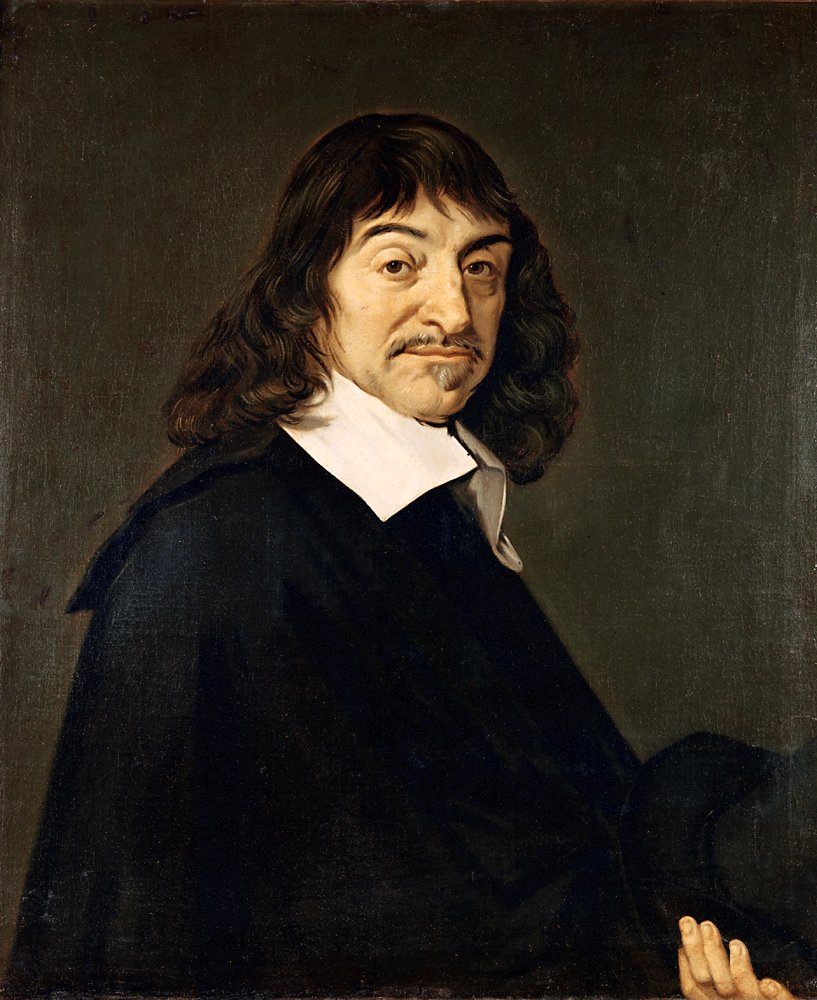
\includegraphics[width = \textwidth]{figures/descartes.jpg}
      
    \end{column}
  \end{columns}
  
\end{frame}

%------------------------------------------------------------------------------%

\begin{frame}{Algebraic Example}
  
  Consider the following equation:
  \begin{align*}
    5 = x + y
  \end{align*}
  What are the values of $x$ and $y$?
  \pause
  \begin{align*}
    y = 5 - x
  \end{align*}
  \pause
  What if we assume that $y = x$?
  \pause
  \begin{align*}
    5 &= x + y\\
    0 &= x - y
  \end{align*}
  \pause
  Now we have enough information:
  \begin{align*}
    5 = x + x = 2x~~\Rightarrow~~x = y = 2.5
  \end{align*}
  
\end{frame}

%------------------------------------------------------------------------------%

\begin{frame}{Assumptions in Statistics}
  
  Why do we need \emph{assumptions} in statistics?
  \begin{itemize}
  \item Data, by themselves, do not offer enough information to support 
    statistical analysis.
    \vc
  \item We need to assume some properties of the population model that generated
    the data.
    \vc
  \item We also use assumptions to simplify problems.
  \end{itemize}
  
\end{frame}

%------------------------------------------------------------------------------%

\begin{frame}{Gauss-Markov Theorem: Setup}
  
  Consider linear regression models of the form:
  \begin{align*}
    Y = \beta_0 + \sum_{p = 1}^P \beta_p X_p + \varepsilon
  \end{align*}
  \vx{-12}
  \begin{itemize}
  \item Assume $\mathbf{X}$ is fixed over repeated sampling.
    \vb
  \item Assume the following properties of the errors:
    \vb
    \begin{enumerate}
    \item The errors have a mean of zero:
      \begin{itemize}
      \item $E[\varepsilon_n] = 0$
      \end{itemize}
      \vb
    \item The errors have constant, finite variance.
      \vc
      \begin{itemize}
      \item $\text{Var}(\varepsilon_n) = \sigma^2 < \infty$
      \end{itemize}
      \vb
    \item The errors are uncorrelated.
      \vc
      \begin{itemize}
      \item $\text{Cov}(\varepsilon_i, \varepsilon_j) = 0, ~ i \neq j$
      \end{itemize}
    \end{enumerate}
  \end{itemize}
  
\end{frame}

%------------------------------------------------------------------------------%

\begin{frame}{Gauss-Markov Theorem}
  
  Given the preceding conditions, the Gauss-Markov Theorem states that the OLS 
  estimates---when they exist---are the \emph{Best Linear Unbiased Estimators} 
  of $\beta$.
  \vc
  \begin{itemize}
  \item OLS estimates are ``best'' in the sense that they will have the lowest 
    variance (i.e., smallest SEs) of any unbiased estimator of $\beta$.
  \end{itemize}
  \vb
  \pause
  Note that the Gauss-Markov Theorem does not require normally distributed 
  errors.
  \vc
  \begin{itemize} 
  \item We assume normally distributed errors to facilitate inference in finite 
    samples.
    \vc
  \item If we assume normally distributed errors, the OLS estimate of $\beta$ is 
    also the \emph{maximum likelihood} estimate.
  \end{itemize}
  
\end{frame}

%------------------------------------------------------------------------------%

\begin{frame}[allowframebreaks]{Assumptions of MLR}

  The typical assumptions for linear regression extend the Gauss-Markov 
  assumptions by:
  \begin{itemize}
  \item Removing the requirement for fixed $\mathbf{X}$
  \item Adding the assumption of normally distributed errors
  \end{itemize}
  \vb
  So, our final assumptions can be stated as follows:
  \vb
  \begin{enumerate}
  \item The model is linear in the parameters.
    \vc
    \begin{itemize}
    \item This is OK: $Y = \beta_0 + \beta_1X + \beta_2Z + \beta_3XZ + \beta_4X^2 + \beta_5X^3 + \varepsilon$
      \vc
    \item This is not: $Y = \beta_0 X^{\beta_1} + \varepsilon$
    \end{itemize}
    \vb
  \item The predictor matrix, $\mathbf{X}$, is \emph{full rank}.  
    \vc
    \begin{itemize}
    \item $N > P$
      \vc
    \item No $X_p$ can be a linear combination of other predictors.
    \end{itemize}
    
    \pagebreak
    
  \item The predictors are strictly exogenous.\label{exo}
    \vc
    \begin{itemize}
    \item The predictors do not correlated with the errors.
      \vc
    \item $\text{Cov}(\mu_{Y|X}, \varepsilon) = 0$
      \vc
    \item $\text{E}(\varepsilon_n|X_n) = 0$
    \end{itemize}
    \vb    
  \item The errors have constant, finite variance.\label{constVar}
    \vc
    \begin{itemize}
    \item $\text{Var}(\varepsilon_n|\mathbf{X}) = \sigma^2 < \infty$
    \end{itemize}
    \vb
  \item The errors are uncorrelated.\label{indErr}
    \vc
    \begin{itemize}
    \item $\text{Cov}(\varepsilon_i, \varepsilon_j|\mathbf{X}) = 0, ~ i \neq j$
    \end{itemize}
    \vb
  \item The errors are normally distributed.\label{normErr}
    \vc
    \begin{itemize}
    \item $\varepsilon|\mathbf{X} \sim \text{N}(0, \sigma^2)$
    \end{itemize}
  \end{enumerate}
  
  \pagebreak
  
  The assumption of \emph{spherical errors} combines Assumptions \ref{constVar} 
  and \ref{indErr}. 
  \begin{align*}
    \text{Var}(\varepsilon|\mathbf{X}) = 
    \begin{bmatrix}
      \sigma^2 & 0 & \cdots & 0\\
      0 & \sigma^2 & \cdots & 0\\
      0 & 0 & \ddots & 0\\
      0 & 0 & \cdots & \sigma^2 
    \end{bmatrix} = 
    \sigma^2\mathbf{I}_N
  \end{align*}
  We can combine Assumptions \ref{exo}, \ref{constVar}, \ref{indErr}, and 
  \ref{normErr} by assuming independent and identically distributed normal 
  errors:
  \begin{itemize}
  \item $\varepsilon|\mathbf{X} \overset{iid}{\sim} \text{N}(0, \sigma^2)$
  \end{itemize}
  \vb
  Keeping the assumptions stated in finer levels of detail, however, is helpful 
  for diagnosing violations.
  \begin{itemize}
  \item We will work with the fine-grained definition of six assumptions.
  \end{itemize}
  
\end{frame}

%------------------------------------------------------------------------------%

\begin{frame}{Consequences of Violating Assumptions}
  
  \begin{enumerate}
  \item If the model is not linear in the parameters, then we're not even 
    working with linear regression.
    \begin{itemize} 
    \item We need to move to entirely different modeling paradigm.
    \end{itemize}
    \vb
  \item If the predictor matrix is not full rank, the model is not estimable.
    \begin{itemize} 
    \item The parameter estimates cannot be uniquely determined from the data.
    \end{itemize}
    \vb
  \item If the predictors are not exogenous, the estimated regression 
    coefficients will be biased.
    \vb
  \item If the errors are not spherical, the standard errors will be biased.
    \begin{itemize}
    \item The estimated regression coefficients will be unbiased, though.
    \end{itemize}
    \vb
  \item If errors are non-normal, small-sample inferences may be biased.
    \begin{itemize}
    \item The justification for some tests and procedures used in regression 
      analysis may not hold.
    \end{itemize}
  \end{enumerate}
  
\end{frame}

%------------------------------------------------------------------------------%

\begin{frame}{Regression Diagnostics}
 
  If some of the assumptions are (grossly) violated, the inferences we make
  using the model may be wrong.  
  \begin{itemize}
  \item We need to check the tenability of our assumptions before leaning too
    heavily on the model estimates.
  \end{itemize}
  \vb
  These checks are called \emph{regression diagnostics}.
  \begin{itemize}
  \item Graphical visualizations
    \vc
  \item Quantitative indices/measures
    \vc
  \item Formal statistical tests
  \end{itemize}
  
\end{frame}

\watermarkoff %----------------------------------------------------------------%

\begin{frame}{Residual Plots}

  One of the most useful diagnostic graphics is the plot of residuals vs. 
  predicted values.

\vb

\begin{columns}
\begin{column}{0.5\textwidth}
      
\begin{knitrout}\footnotesize
\definecolor{shadecolor}{rgb}{0.878, 0.918, 0.933}\color{fgcolor}

{\centering 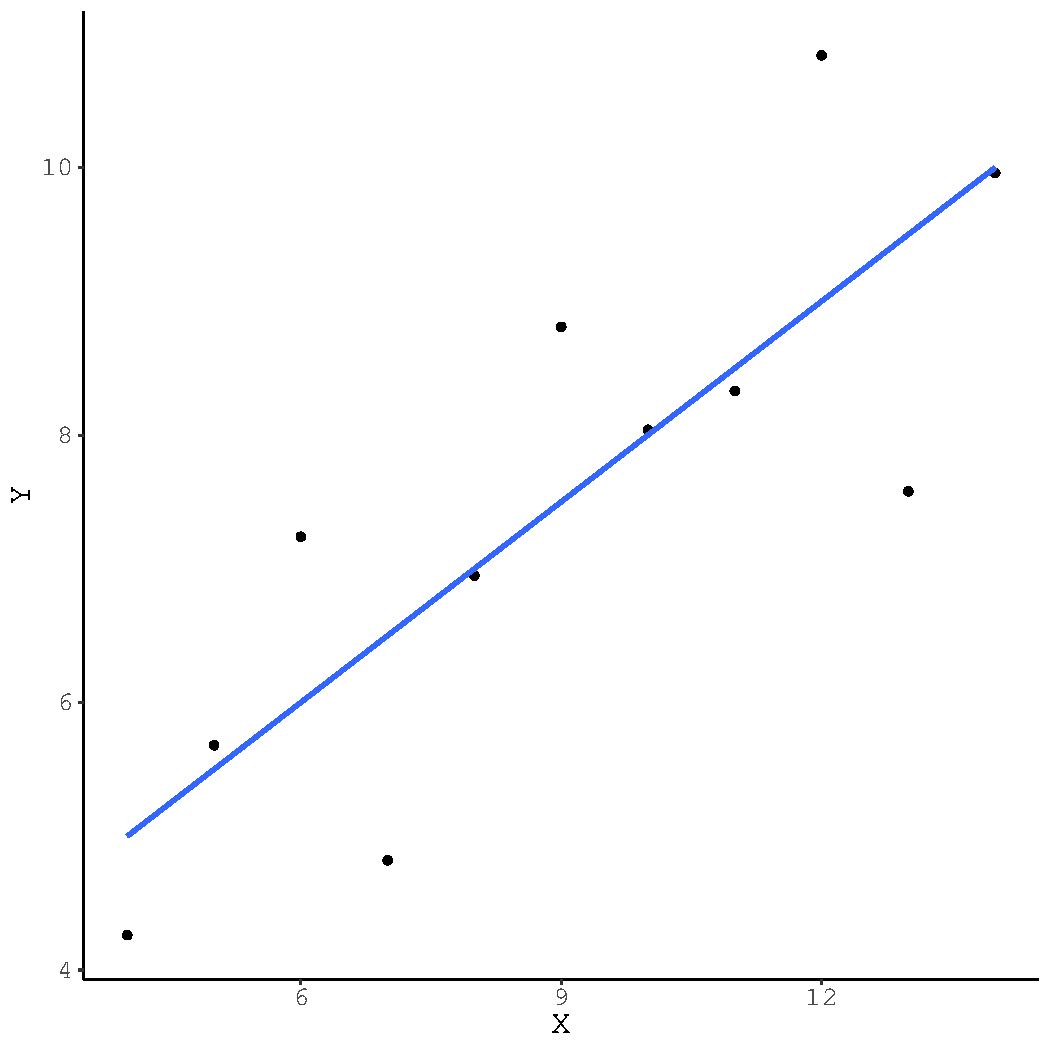
\includegraphics[width=\maxwidth]{figure/unnamed-chunk-1-1} 

}



\end{knitrout}
\end{column}
    
\begin{column}{0.5\textwidth}
      
\begin{knitrout}\footnotesize
\definecolor{shadecolor}{rgb}{0.878, 0.918, 0.933}\color{fgcolor}

{\centering 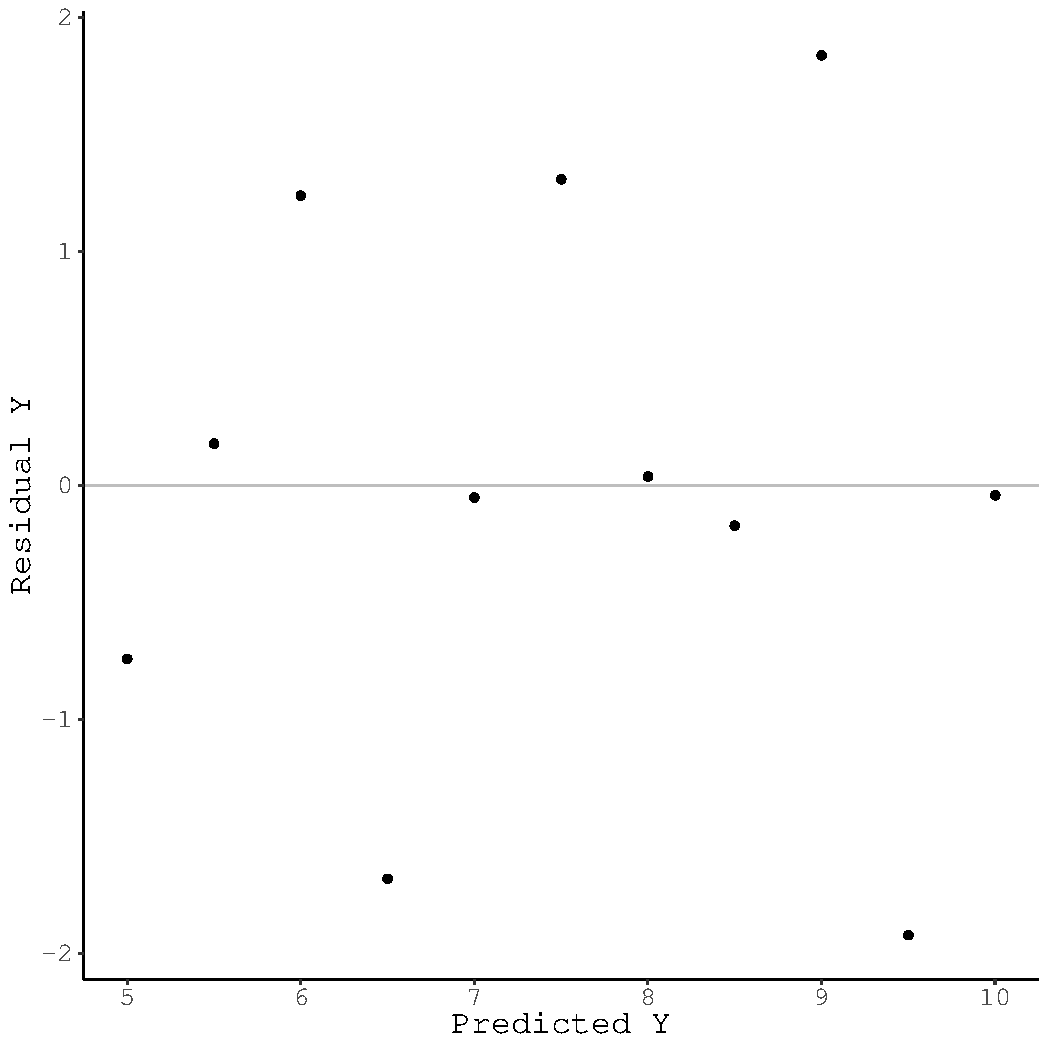
\includegraphics[width=\maxwidth]{figure/unnamed-chunk-2-1} 

}



\end{knitrout}

\end{column}
\end{columns}

\end{frame}

%------------------------------------------------------------------------------%

\begin{frame}{Residual Plots}
  
  Recall the Anscombe data that we saw when discussing EDA:
  \va

\begin{knitrout}\footnotesize
\definecolor{shadecolor}{rgb}{0.878, 0.918, 0.933}\color{fgcolor}

{\centering 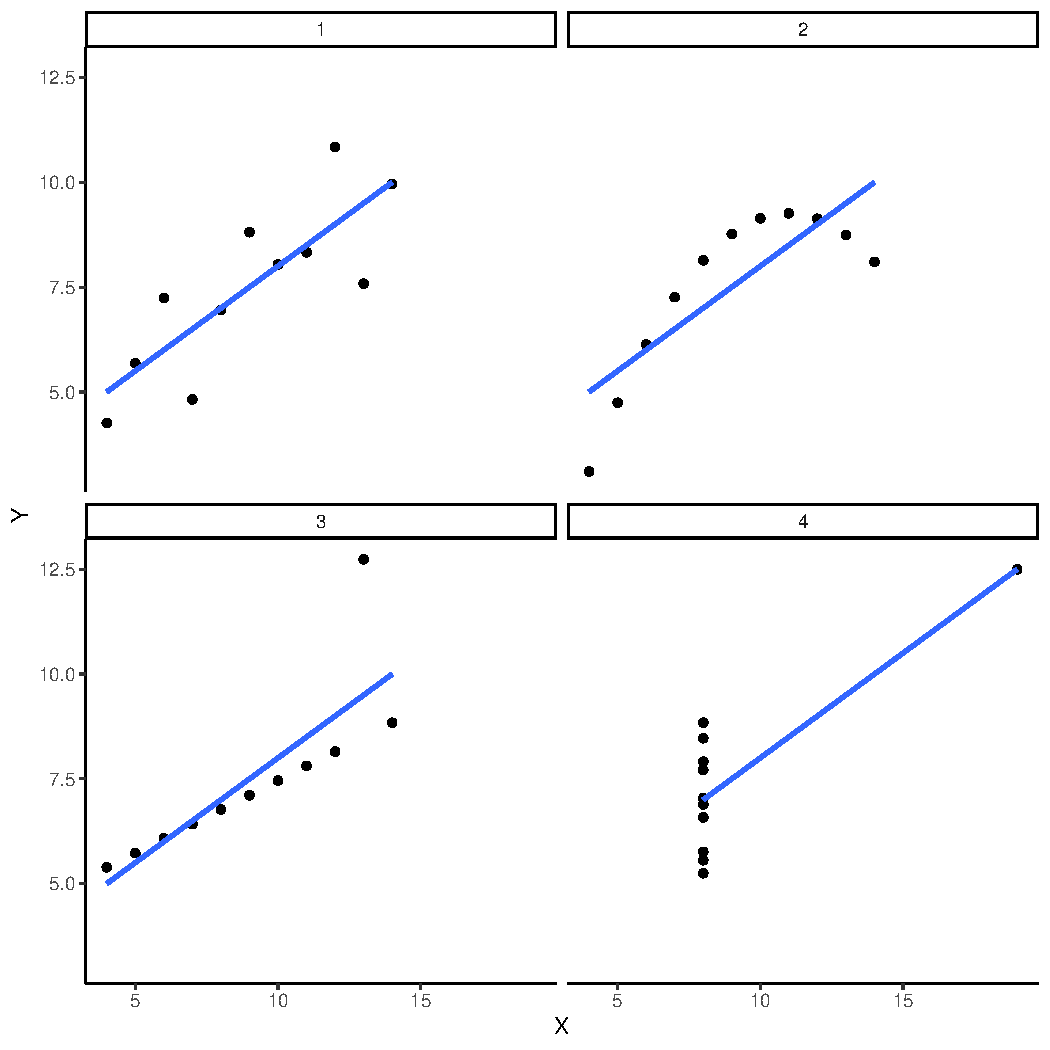
\includegraphics[width=0.5\linewidth]{figure/unnamed-chunk-3-1} 

}



\end{knitrout}
 
\end{frame}

%------------------------------------------------------------------------------%

\begin{frame}{Residual Plots}
  
  The residual plots clearly highlight the problems:

\va

\begin{knitrout}\footnotesize
\definecolor{shadecolor}{rgb}{0.878, 0.918, 0.933}\color{fgcolor}

{\centering 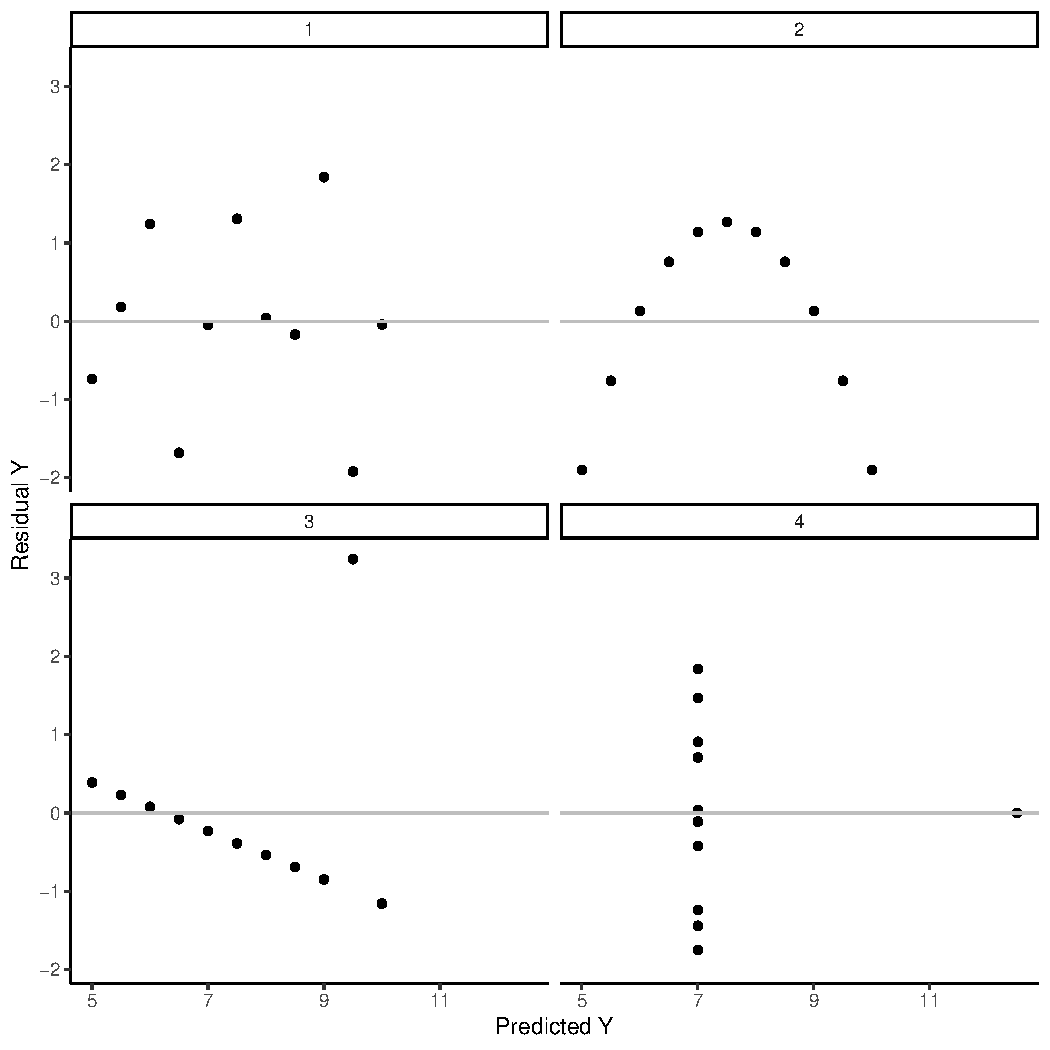
\includegraphics[width=0.5\linewidth]{figure/unnamed-chunk-4-1} 

}



\end{knitrout}

\end{frame}

%------------------------------------------------------------------------------%

\begin{frame}{Heteroscedasticity}
  
  One commonly encountered problem is non-constant error variance (i.e., 
  \emph{heteroscedasticity}) which violates Assumption \ref{constVar}.
  \vb
  \begin{columns}
    \begin{column}{0.5\textwidth}
      
\begin{knitrout}\footnotesize
\definecolor{shadecolor}{rgb}{0.878, 0.918, 0.933}\color{fgcolor}

{\centering 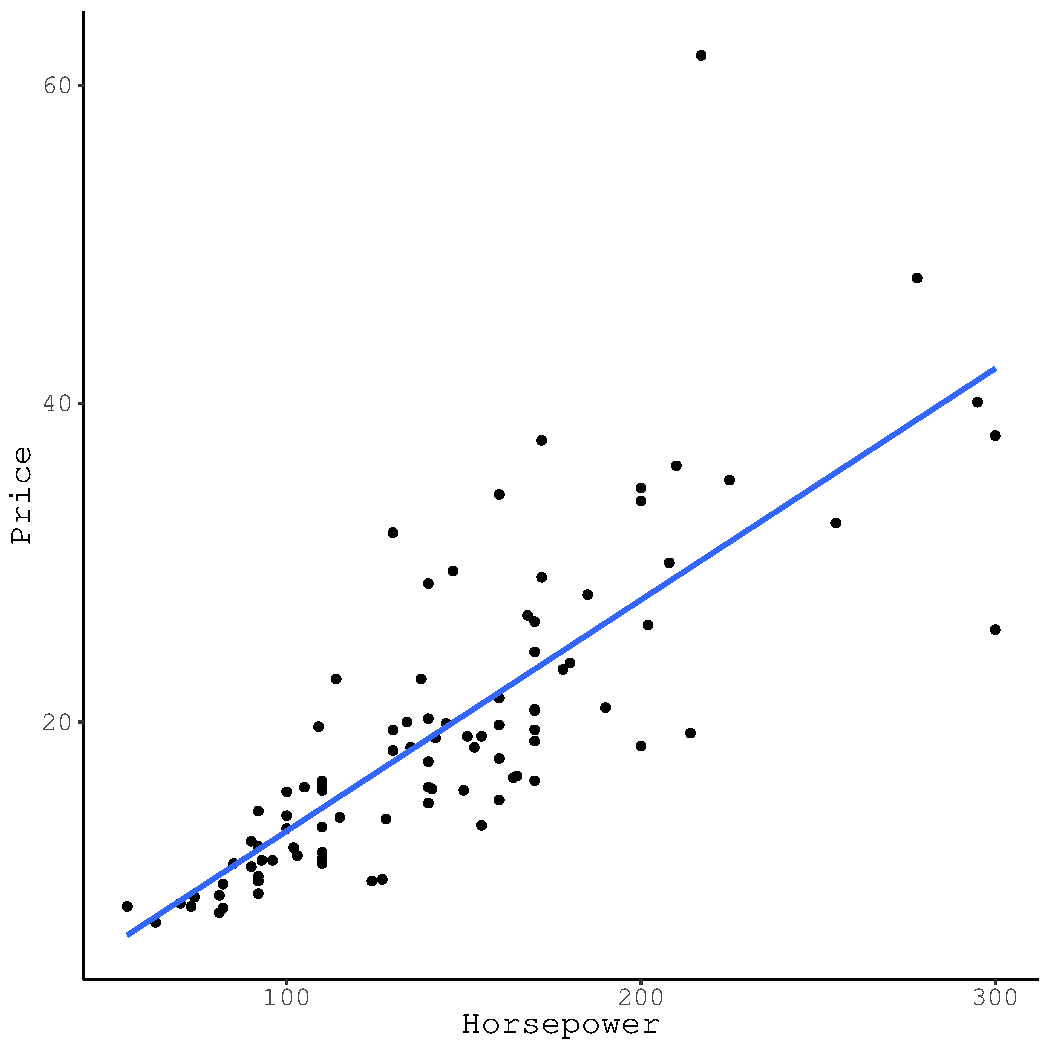
\includegraphics[width=\maxwidth]{figure/unnamed-chunk-5-1} 

}



\end{knitrout}
\end{column}
    
    \begin{column}{0.5\textwidth}
      
\begin{knitrout}\footnotesize
\definecolor{shadecolor}{rgb}{0.878, 0.918, 0.933}\color{fgcolor}

{\centering 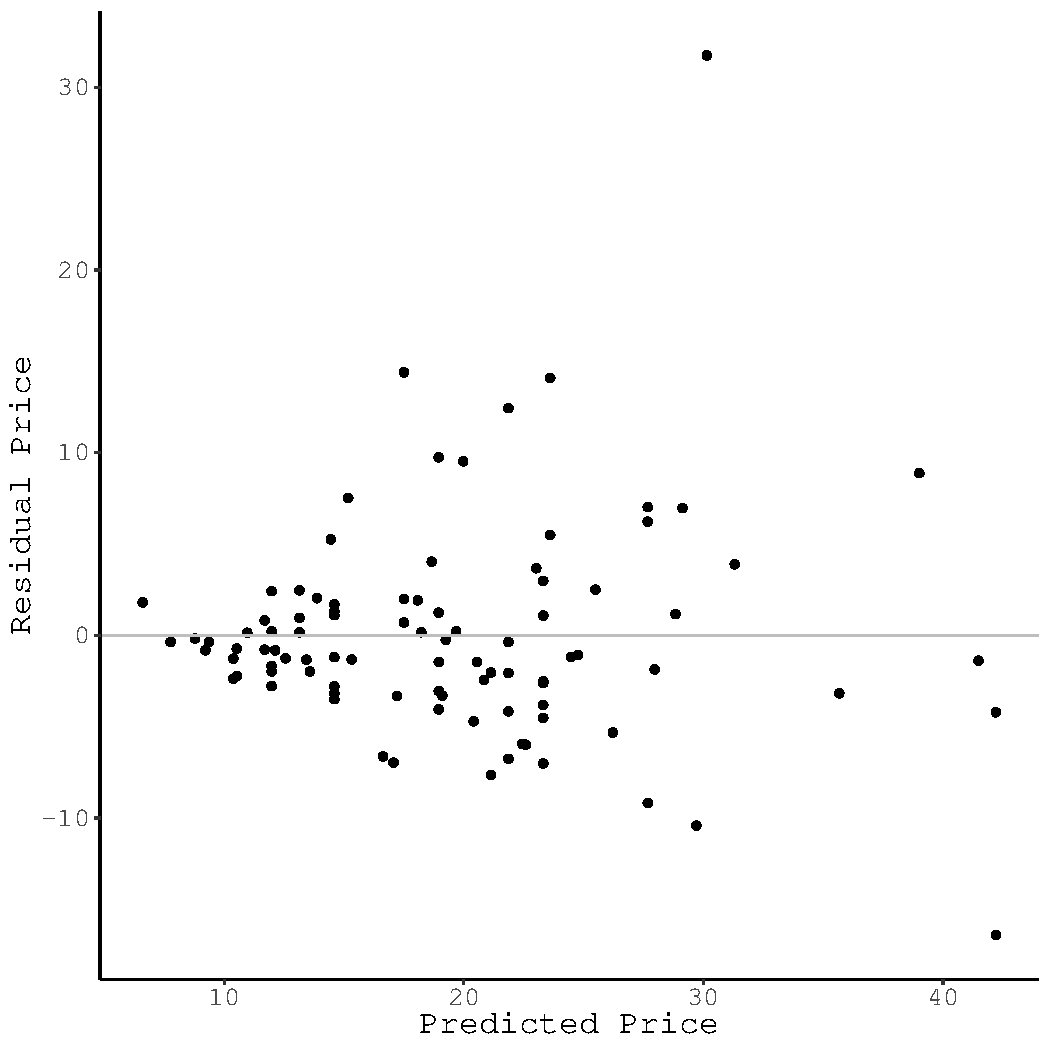
\includegraphics[width=\maxwidth]{figure/unnamed-chunk-6-1} 

}



\end{knitrout}

\end{column}
\end{columns}

\end{frame}

\watermarkon %-----------------------------------------------------------------%

\begin{frame}{Testing for Heteroscedasticity}
  
  Residual plots---like the one shown on the last slide---are probably the best 
  way to detect potential heteroscedasticity, but we can also do statistical 
  tests.
  \vb
  \begin{itemize}
  \item When heteroscedasticity is present, the variance of the residuals will 
    vary along the regression line.
    \vc
  \item If the pattern of this change is approximately monotonic, we can detect 
    it by regression an estimate of the pointwise residual variance onto the 
    predictors.
    \vc
    \begin{itemize}
    \item This is the intuition for the \emph{Breusch-Pagan Test}.
      \begin{align*}
        \hat{\varepsilon}^2 = \gamma_0 + \sum_{p = 1}^P \gamma_p X_p + \omega
      \end{align*}
    \end{itemize}
  \end{itemize}
  
\end{frame}

\watermarkoff %----------------------------------------------------------------%

\begin{frame}[fragile]{Example}
  
  Let's apply the Breusch-Pagan Test to the regression we plotted above.
  
\begin{knitrout}\footnotesize
\definecolor{shadecolor}{rgb}{0.878, 0.918, 0.933}\color{fgcolor}\begin{kframe}
\begin{alltt}
\hlkwd{suppressMessages}\hlstd{(}\hlkwd{library}\hlstd{(lmtest))}
\hlkwd{data}\hlstd{(Cars93)}

\hlstd{out1} \hlkwb{<-} \hlkwd{lm}\hlstd{(Price} \hlopt{~} \hlstd{Horsepower,} \hlkwc{data} \hlstd{= Cars93)}
\hlkwd{bptest}\hlstd{(out1)}
\end{alltt}
\begin{verbatim}
## 
## 	studentized Breusch-Pagan test
## 
## data:  out1
## BP = 7.9292, df = 1, p-value = 0.004864
\end{verbatim}
\end{kframe}
\end{knitrout}

We have a significant test statistic, so we reject the null hypothesis of 
homoscedasticity.

\end{frame}

%------------------------------------------------------------------------------%

\begin{frame}{Limitations of the Breusch-Pagan Test}
  
  The Breusch-Pagan test can have trouble detecting non-monotonic 
  heteroscedasticity.
  
  \begin{columns}
    \begin{column}{0.5\textwidth}
      
      
\begin{knitrout}\footnotesize
\definecolor{shadecolor}{rgb}{0.878, 0.918, 0.933}\color{fgcolor}

{\centering 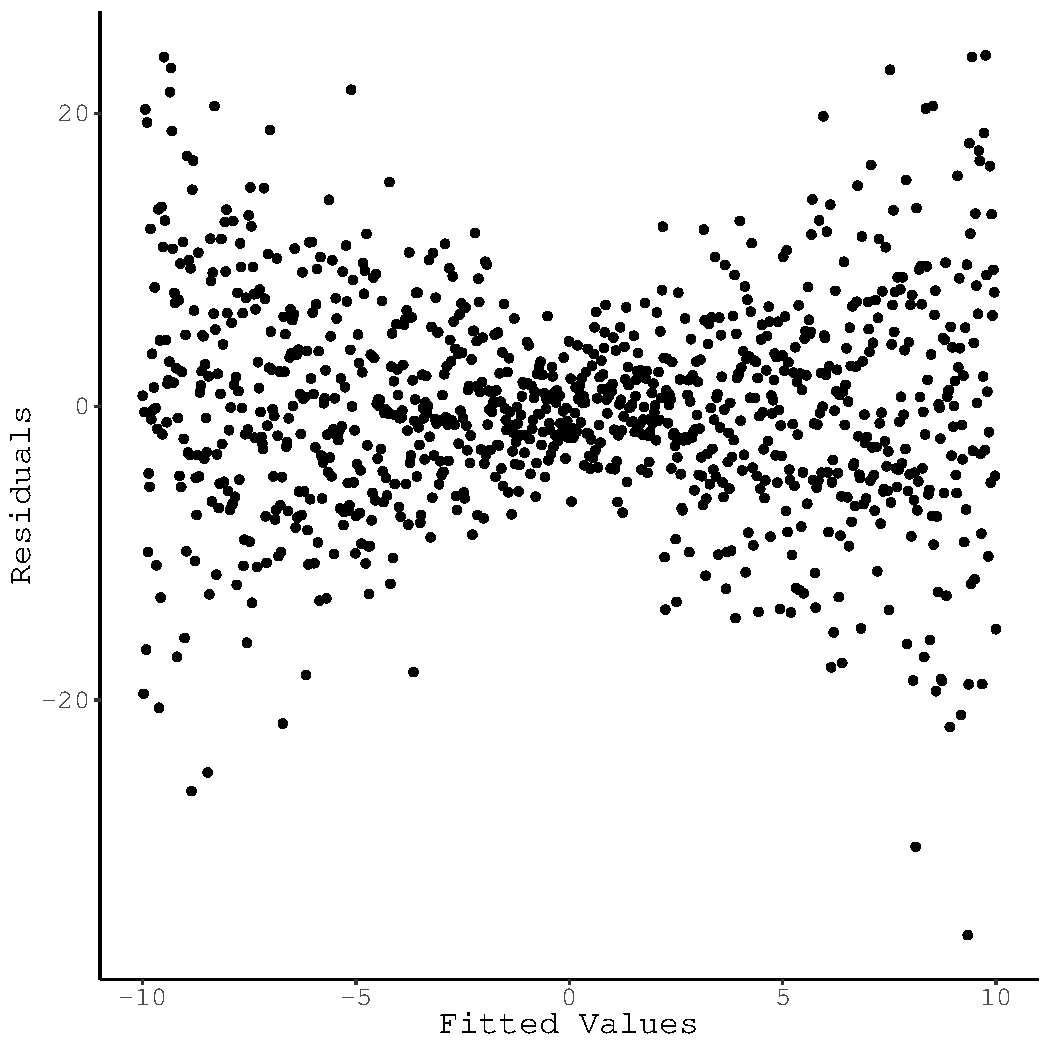
\includegraphics[width=\maxwidth]{figure/unnamed-chunk-8-1} 

}



\end{knitrout}
      
    \end{column}
    
    \begin{column}{0.5\textwidth}
      
\begin{knitrout}\footnotesize
\definecolor{shadecolor}{rgb}{0.878, 0.918, 0.933}\color{fgcolor}

{\centering 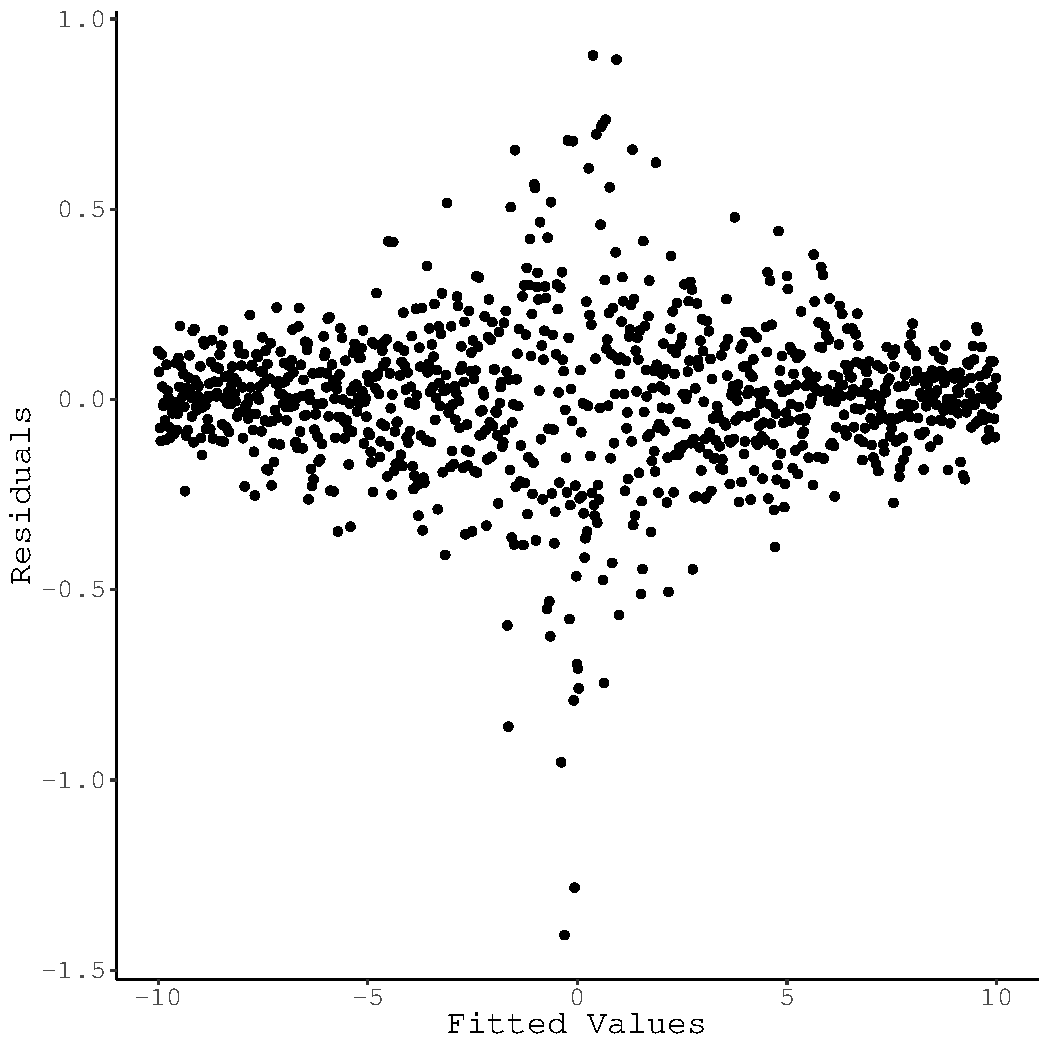
\includegraphics[width=\maxwidth]{figure/unnamed-chunk-9-1} 

}



\end{knitrout}

    \end{column}
  \end{columns}
  
\end{frame}
  
\watermarkon %-----------------------------------------------------------------%

\begin{frame}{Consequences of Heteroscedasticity}
  
  Non-constant error variance will not bias the parameter estimates.
  \begin{itemize}
  \item The best fit line is still correct.
  \item Our measure of uncertainty around that best fit line is wrong.
  \end{itemize}
  \vb
  Heteroscedasticity will bias standard errors (usually downward).
  \begin{itemize}
  \item Test statistics will be too large.
  \item CIs will be too narrow.
  \item We will have inflated Type I error rates.
  \end{itemize}
  \vb
  To get valid inference, we need to address (severe) heteroscedasticity.
  
\end{frame}

%------------------------------------------------------------------------------%

\begin{frame}{Treating Heteroscedasticity}
  
  \begin{enumerate}
  \item Transform your outcome using a concave function (e.g., $\ln(Y)$,
    $\sqrt{Y}$).  
    \vc
    \begin{itemize}
    \item These transformations will shrink extreme values more than
      small/moderate ones.
    \end{itemize}
    \vb
  \item Refit the model using \emph{weighted least squares}.
    \vc
    \begin{itemize}
    \item Create inverse weights using functions of the residual variances or
      quantities highly correlated therewith.
    \end{itemize}
    \vb
  \item Use a \emph{Heteroscedasticity Consistent} (HC) estimate of the 
    asymptotic covariance matrix. 
    \vc
    \begin{itemize}
    \item Robust standard errors, Huber-White standard errors, Sandwich 
      estimators
    \item HC estimators correct the standard errors for non-constant error 
      variance.
    \end{itemize}
  \end{enumerate}
  
\end{frame}

\watermarkoff %----------------------------------------------------------------%

\begin{frame}[fragile, allowframebreaks]{Example}
  
\begin{knitrout}\footnotesize
\definecolor{shadecolor}{rgb}{0.878, 0.918, 0.933}\color{fgcolor}\begin{kframe}
\begin{alltt}
\hlcom{## The 'sandwich' package provides several HC estimators:}
\hlkwd{library}\hlstd{(sandwich)}

\hlcom{## Use sandwich estimator to compute ACOV matrix:}
\hlstd{hcCov} \hlkwb{<-} \hlkwd{vcovHC}\hlstd{(out1)}

\hlcom{## Test coefficients with robust SEs:}
\hlstd{robTest} \hlkwb{<-} \hlkwd{coeftest}\hlstd{(out1,} \hlkwc{vcov} \hlstd{= hcCov)}

\hlcom{## Test coefficients with default SEs:}
\hlstd{defTest} \hlkwb{<-} \hlkwd{summary}\hlstd{(out1)}\hlopt{$}\hlstd{coefficients}
\end{alltt}
\end{kframe}
\end{knitrout}

\pagebreak

\begin{knitrout}\footnotesize
\definecolor{shadecolor}{rgb}{0.878, 0.918, 0.933}\color{fgcolor}\begin{kframe}
\begin{alltt}
\hlcom{## Compare robust and default approaches:}
\hlstd{robTest}
\end{alltt}
\begin{verbatim}
## 
## t test of coefficients:
## 
##              Estimate Std. Error t value  Pr(>|t|)
## (Intercept) -1.398769   2.078200 -0.6731    0.5026
## Horsepower   0.145371   0.017164  8.4696 4.051e-13
\end{verbatim}
\begin{alltt}
\hlstd{defTest}
\end{alltt}
\begin{verbatim}
##               Estimate Std. Error    t value     Pr(>|t|)
## (Intercept) -1.3987691  1.8200164 -0.7685475 4.441519e-01
## Horsepower   0.1453712  0.0118978 12.2183251 6.837464e-21
\end{verbatim}
\end{kframe}
\end{knitrout}

\end{frame}

\watermarkon %-----------------------------------------------------------------%

\begin{frame}{Correlated Errors}
  
  Errors can become correlated in two basic ways:
  \vb
  \begin{enumerate}
  \item Serial dependence
    \begin{itemize}
    \item When modeling longitudinal data, the errors for a given observational 
      unit are correlated over time.
      \vc
    \item We can detect temporal dependence by examining the 
      \emph{autocorrelation} of the residuals.
    \end{itemize}
    \vb
  \item Clustering
    \begin{itemize}
    \item Your data have some important, unmodeled, grouping structure.
      \begin{itemize}
      \item Children nested within classrooms
      \item Romantic couples
      \item Departments within a company
      \end{itemize}
      \vc
    \item We can detect problematic levels of clustering with the 
      \emph{intraclass correlation coefficient} (ICC).
      \begin{itemize}
      \item We need to know the clustering variable to apply the ICC.
      \end{itemize}
    \end{itemize}
  \end{enumerate}
  
\end{frame}

%------------------------------------------------------------------------------%

\begin{frame}[allowframebreaks]{Treating Correlated Errors}
  
  Serially dependent errors in a longitudinal model usually indicate an 
  inadequate model.
  \vc
  \begin{itemize}
  \item Your model is ignoring some important aspect of the temporal variation 
    that is being absorbed by the error terms.
    \vc
  \item Hopefully, you can add the missing component to your model.
  \end{itemize}
  
  \pagebreak
  
  Clustering can be viewed as theoretically meaningful or as a nuisance factor 
  that just needs to be controlled.
  \vb
  \begin{itemize}
  \item If the clustering is meaningful, you should model the data using 
    \emph{multilevel modeling}.
    \vc
    \begin{itemize}
    \item Hierarchical linear regression
      \vc
    \item Mixed models
      \vc
    \item Random effects models
    \end{itemize}
    \vc
  \item If the clustering is an uninteresting nuisance, you can use specialized 
    HC variance estimators that deal with clustering.
  \end{itemize}
  
\end{frame}
  
\watermarkoff %----------------------------------------------------------------%

\begin{frame}{Model Specification}

  Our assumptions mostly focus on the errors, so incorrect model specification 
  can lead to violations of many assumptions. 
  \vb
  \begin{columns}
    \begin{column}{0.5\textwidth}
      
\begin{knitrout}\footnotesize
\definecolor{shadecolor}{rgb}{0.878, 0.918, 0.933}\color{fgcolor}

{\centering 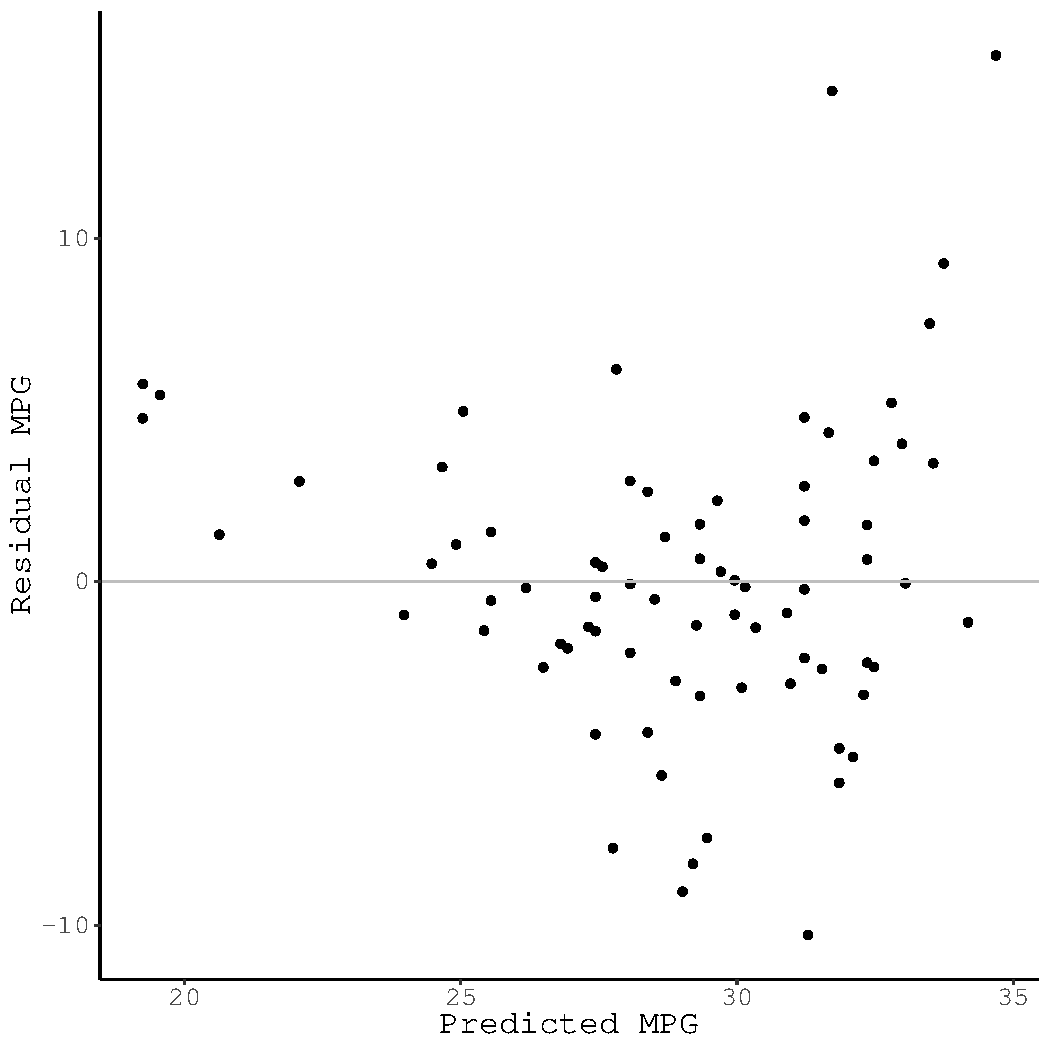
\includegraphics[width=\maxwidth]{figure/unnamed-chunk-12-1} 

}



\end{knitrout}

\end{column}

\begin{column}{0.5\textwidth}
      
\begin{knitrout}\footnotesize
\definecolor{shadecolor}{rgb}{0.878, 0.918, 0.933}\color{fgcolor}

{\centering 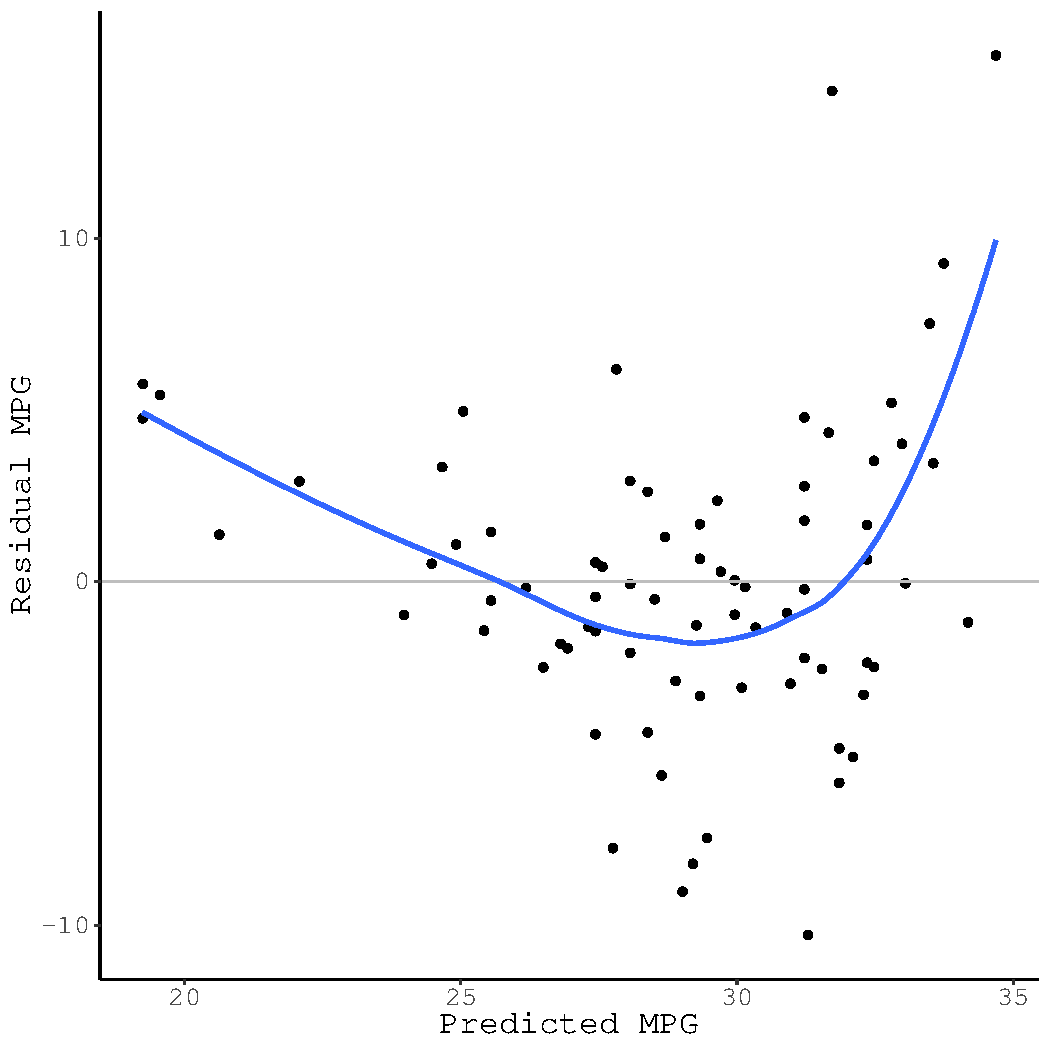
\includegraphics[width=\maxwidth]{figure/unnamed-chunk-13-1} 

}



\end{knitrout}

\end{column}
\end{columns}
  
\end{frame}

%------------------------------------------------------------------------------%

\begin{frame}{Nonlinear Trends in Residual Plots}

  Clearly, the linear trend fits these data poorly.
  \begin{itemize}
    \item We should probably add some polynomial terms
  \end{itemize}
  \vb
  \begin{columns}
    \begin{column}{0.5\textwidth}
      
\begin{knitrout}\footnotesize
\definecolor{shadecolor}{rgb}{0.878, 0.918, 0.933}\color{fgcolor}

{\centering 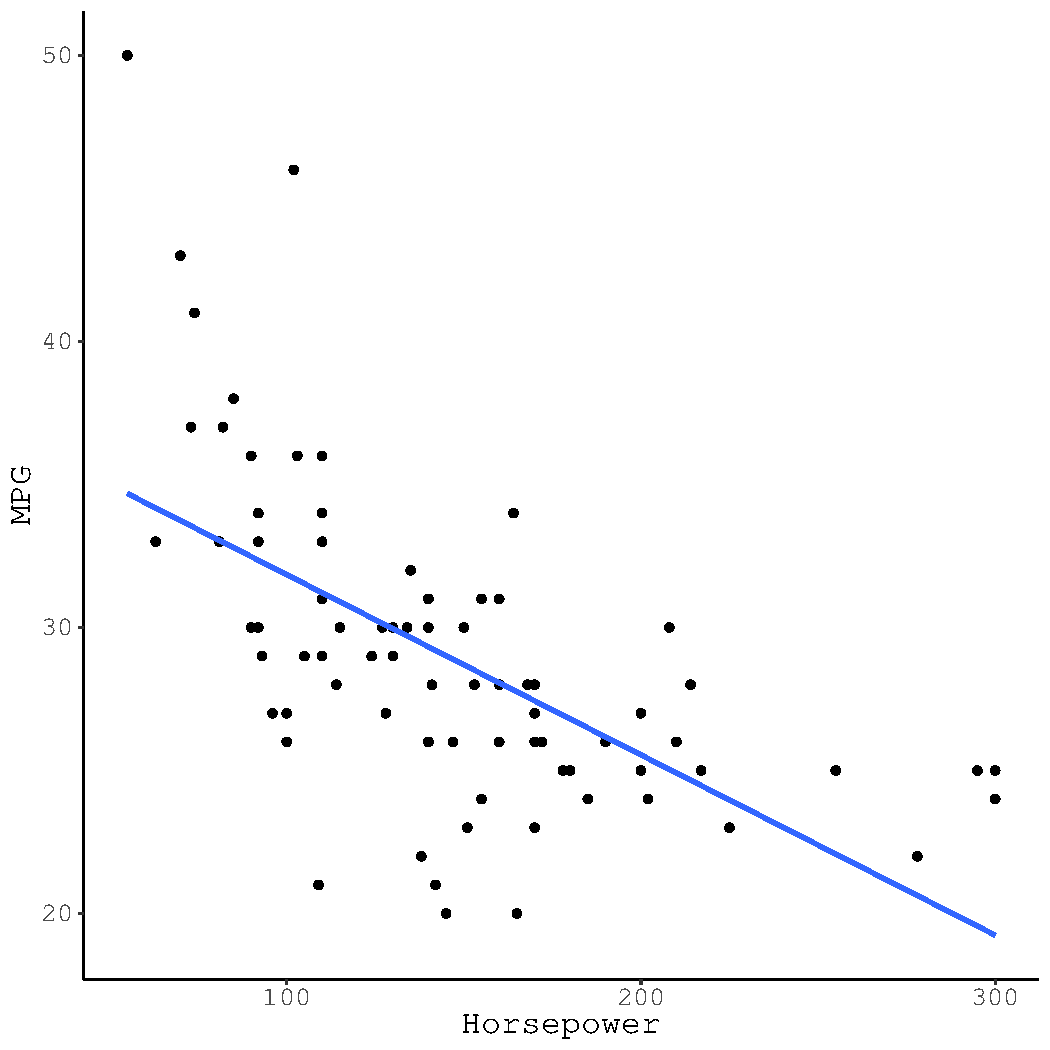
\includegraphics[width=\maxwidth]{figure/unnamed-chunk-14-1} 

}



\end{knitrout}

\end{column}

\begin{column}{0.5\textwidth}
      
\begin{knitrout}\footnotesize
\definecolor{shadecolor}{rgb}{0.878, 0.918, 0.933}\color{fgcolor}

{\centering 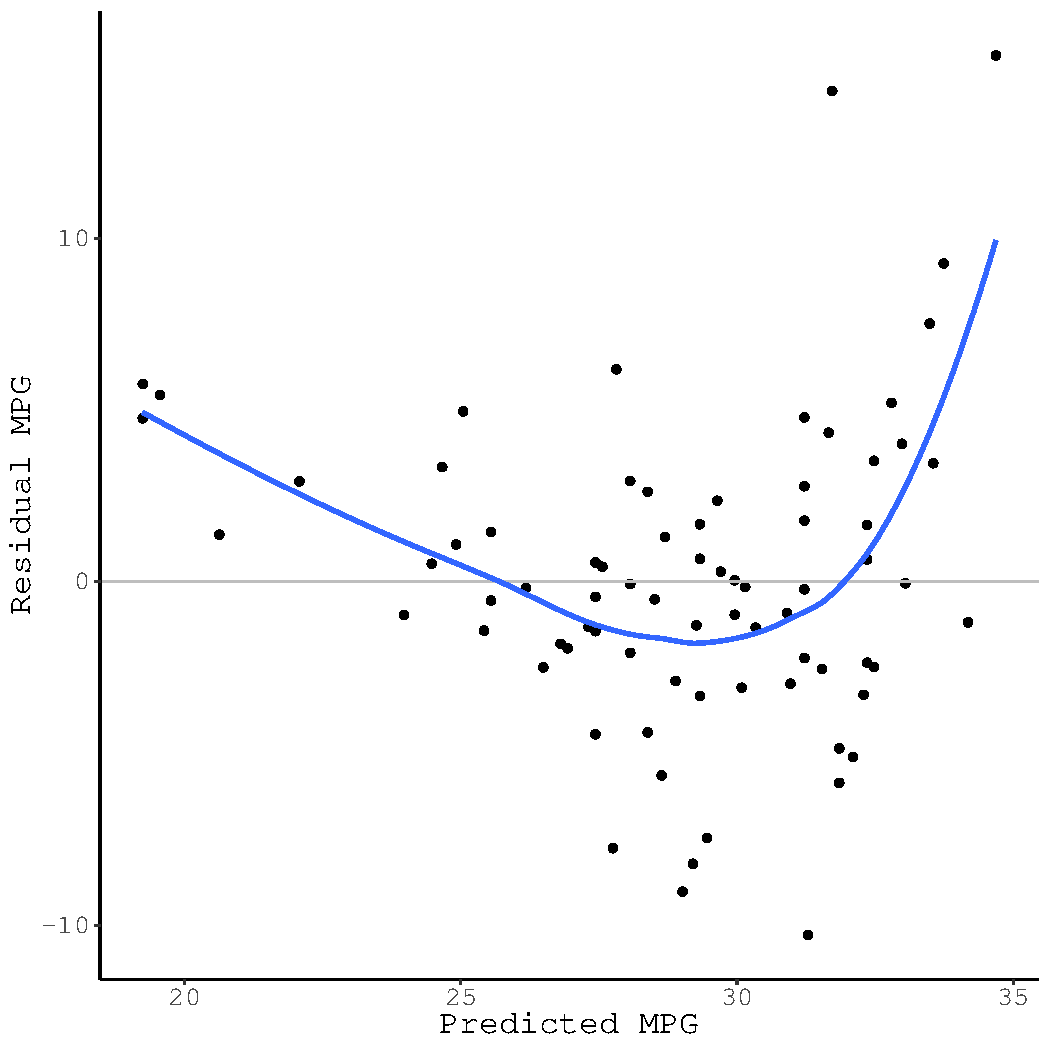
\includegraphics[width=\maxwidth]{figure/unnamed-chunk-15-1} 

}



\end{knitrout}

\end{column}
\end{columns}
  
\end{frame}

\watermarkon %-----------------------------------------------------------------%

\begin{frame}{Treating Residual Nonlinearity}
  
  Nonlinearity in the residual plots is usually a sign of either:
  \begin{enumerate}
  \item Model misspecification
  \item Influential observations
  \end{enumerate}
  \vb 
  This type of model misspecification usually implies omitted functions of 
  modeled variables.  
  \begin{itemize}
  \item Polynomial terms
  \item Interactions
  \end{itemize}
  \vb
  The solution is to include the omitted term into the model and refit.
  \begin{itemize}
  \item This is very much easier said than done.
  \end{itemize}
  
\end{frame}

\watermarkoff %----------------------------------------------------------------%

\begin{frame}{Residual Plots}

  Certainly looks better, but not ideal.
  \vb
  \begin{columns}
    \begin{column}{0.5\textwidth}
      
\begin{knitrout}\footnotesize
\definecolor{shadecolor}{rgb}{0.878, 0.918, 0.933}\color{fgcolor}

{\centering 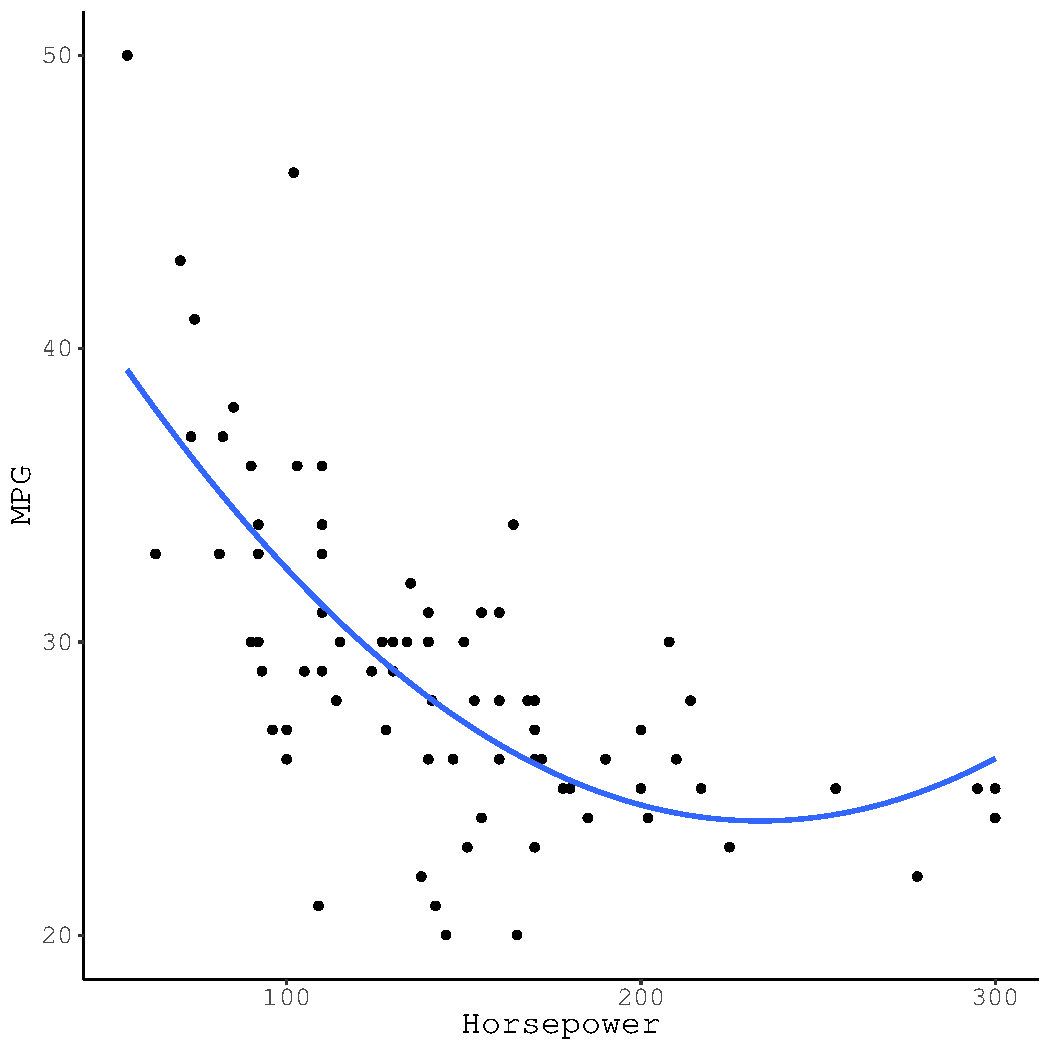
\includegraphics[width=\maxwidth]{figure/unnamed-chunk-16-1} 

}



\end{knitrout}

\end{column}

\begin{column}{0.5\textwidth}
      
\begin{knitrout}\footnotesize
\definecolor{shadecolor}{rgb}{0.878, 0.918, 0.933}\color{fgcolor}

{\centering 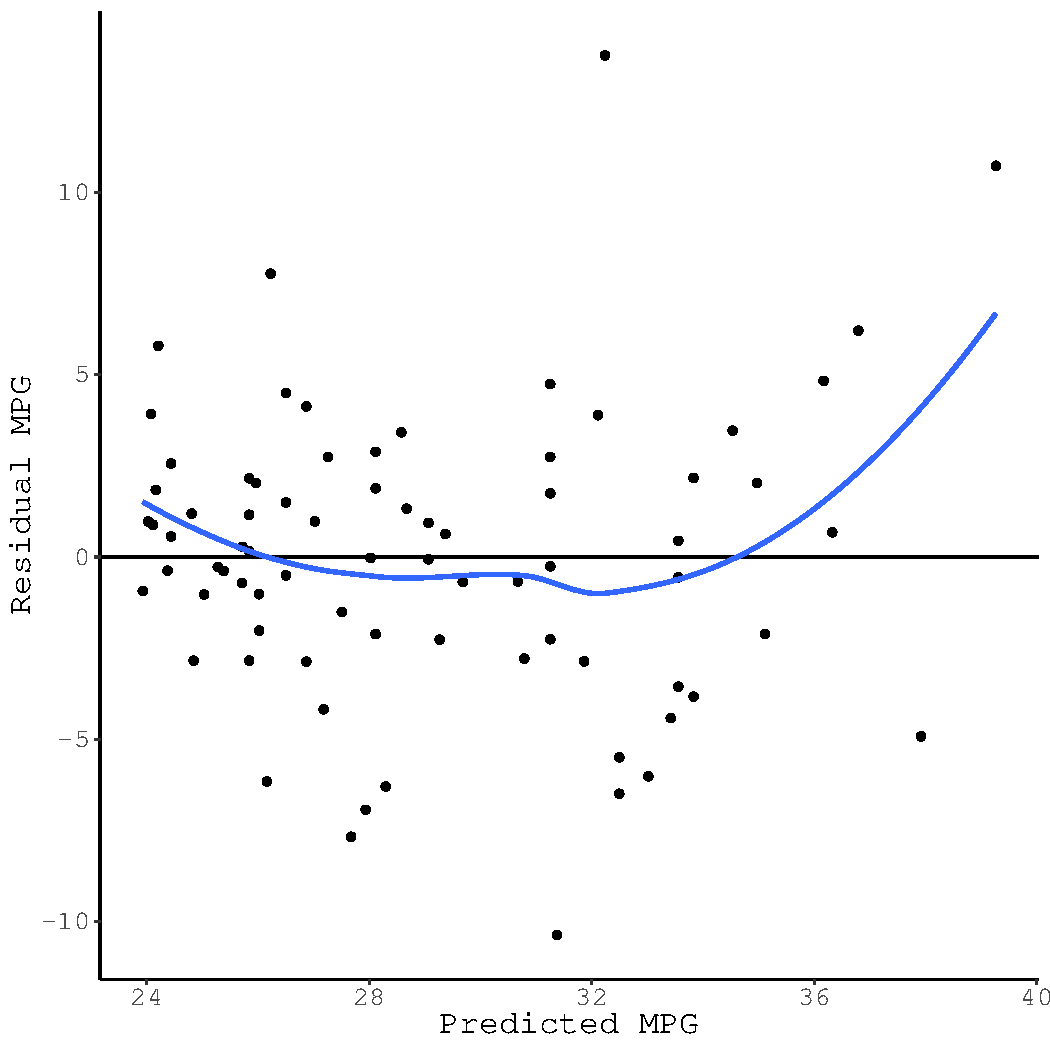
\includegraphics[width=\maxwidth]{figure/unnamed-chunk-17-1} 

}



\end{knitrout}

\end{column}
\end{columns}
  
\end{frame}

%------------------------------------------------------------------------------%

\begin{frame}{Residual Plots}

  Further improvement (perhaps).
  \vb
  \begin{columns}
    \begin{column}{0.5\textwidth}
      
\begin{knitrout}\footnotesize
\definecolor{shadecolor}{rgb}{0.878, 0.918, 0.933}\color{fgcolor}

{\centering 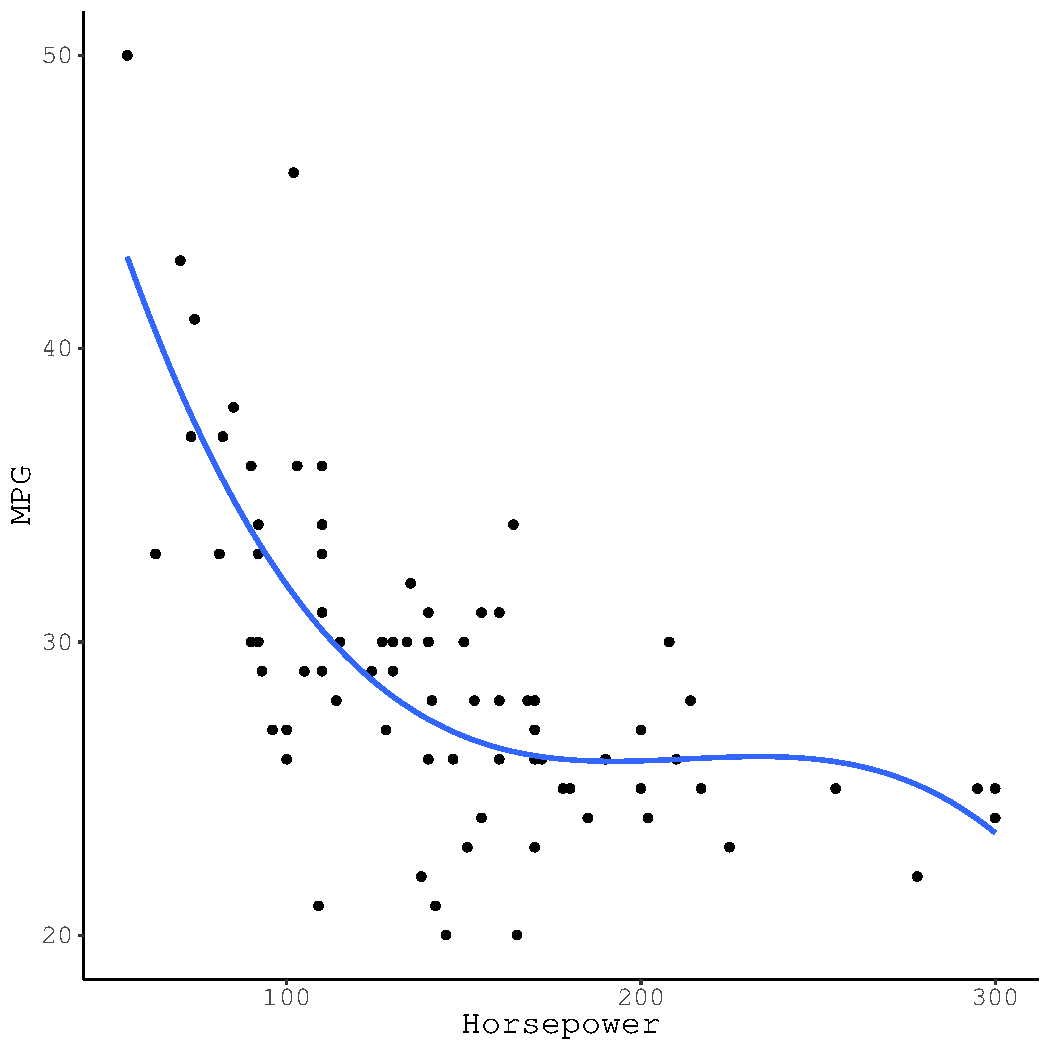
\includegraphics[width=\maxwidth]{figure/unnamed-chunk-18-1} 

}



\end{knitrout}

\end{column}

\begin{column}{0.5\textwidth}
  
\begin{knitrout}\footnotesize
\definecolor{shadecolor}{rgb}{0.878, 0.918, 0.933}\color{fgcolor}

{\centering 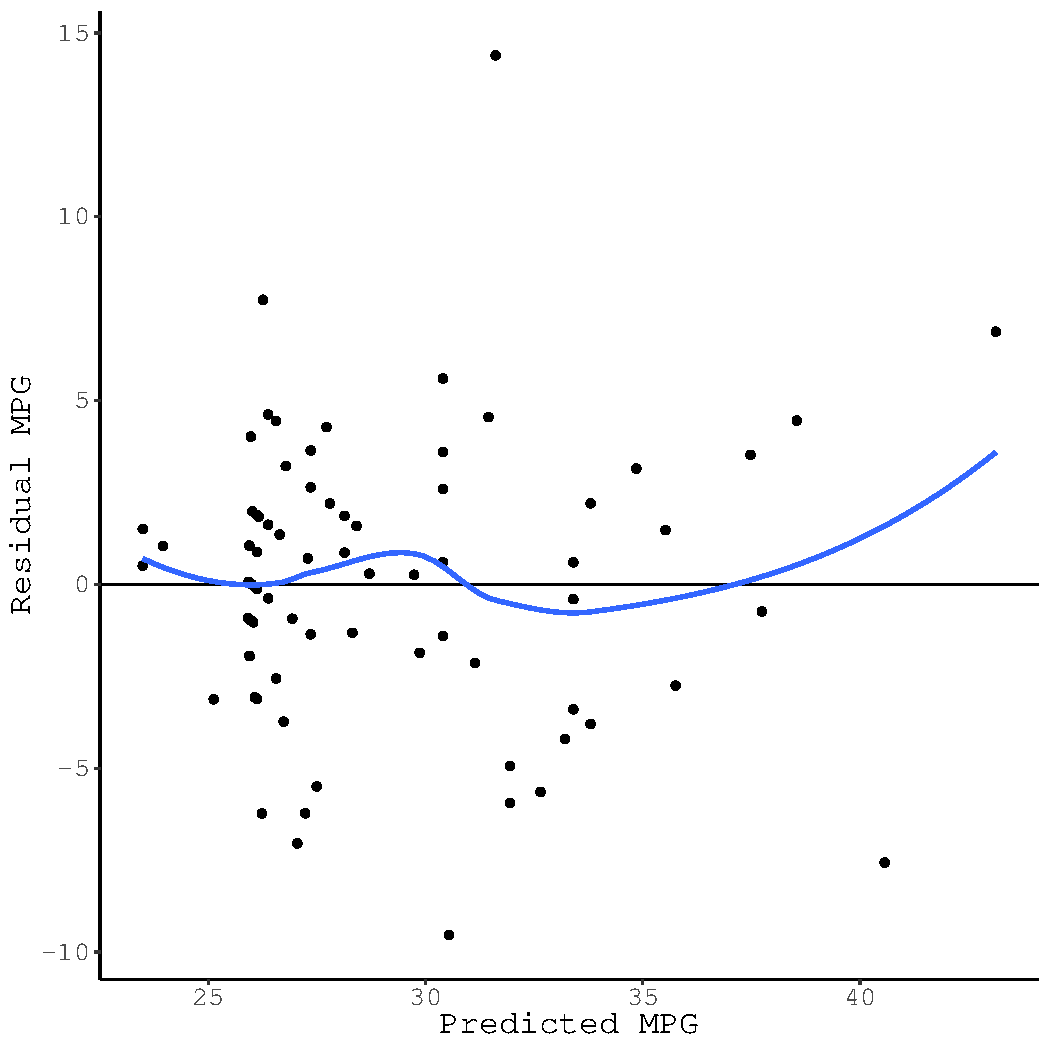
\includegraphics[width=\maxwidth]{figure/unnamed-chunk-19-1} 

}



\end{knitrout}

\end{column}
\end{columns}
  
\end{frame}

\watermarkon %-----------------------------------------------------------------%

\begin{frame}{Model Specification Tests}
  
  As with heteroscedasticity, residual plots are probably the best way to assess 
  model misspecification, but we can do statistical tests here, too.
  \vb
  \begin{itemize}
  \item One of the most popular specification tests is the Ramsey 
    \emph{Regression Equation Specification Error Test} (RESET).
    \vb
  \item If the functional form of the model is misspecified, then including 
    additional nonlinear predictors should improve fit.
    \vc
    \begin{itemize}
    \item In particular, we usually including polynomial transformations of the 
      predictors or the fitted values.
    \end{itemize}
  \end{itemize}
  
\end{frame}

%------------------------------------------------------------------------------%

\begin{frame}{Ramsey RESET}
  
  Given the estimated model:
  \begin{align*}
    Y = \hat{\beta}_0 + \sum_{p = 1}^P \hat{\beta}_pX_p + \hat{\varepsilon}
  \end{align*}
  We'll estimated the augmented model:
  \begin{align*}
    Y = \hat{\beta}_0 + \sum_{p = 1}^P \hat{\beta}_pX_p + \sum_{q = 1}^Q \hat{\gamma}_q Z_q + \hat{\varepsilon}
  \end{align*}
  Then we check if the augmented model fits better than the original.
  \begin{itemize}
  \item The $Z_q$ are usually taken to be powers of $X_p$ or $\hat{Y}$.
  \item If the augmented model fits better, we reject the null hypothesis of 
    correct specification.
  \end{itemize}
  
\end{frame}

\watermarkoff %----------------------------------------------------------------%

\begin{frame}[fragile]{Example}

  Let's apply the RESET to the model plotted above:
\begin{knitrout}\footnotesize
\definecolor{shadecolor}{rgb}{0.878, 0.918, 0.933}\color{fgcolor}\begin{kframe}
\begin{alltt}
\hlstd{out2} \hlkwb{<-} \hlkwd{lm}\hlstd{(MPG.highway} \hlopt{~} \hlstd{Horsepower,} \hlkwc{data} \hlstd{= Cars93)}

\hlkwd{resettest}\hlstd{(out2)}
\end{alltt}
\begin{verbatim}
## 
## 	RESET test
## 
## data:  out2
## RESET = 16.718, df1 = 2, df2 = 89, p-value =
## 6.852e-07
\end{verbatim}
\end{kframe}
\end{knitrout}

The test definitely suggests misspecification.

\end{frame}

%------------------------------------------------------------------------------%

\begin{frame}[fragile]{Example}

  What happens when we add the square of horsepower?
  
\begin{knitrout}\footnotesize
\definecolor{shadecolor}{rgb}{0.878, 0.918, 0.933}\color{fgcolor}\begin{kframe}
\begin{alltt}
\hlstd{out3} \hlkwb{<-} \hlkwd{update}\hlstd{(out2,} \hlstr{". ~ . + I(Horsepower^2)"}\hlstd{)}
\hlkwd{resettest}\hlstd{(out3)}
\end{alltt}
\begin{verbatim}
## 
## 	RESET test
## 
## data:  out3
## RESET = 5.1653, df1 = 2, df2 = 88, p-value = 0.007567
\end{verbatim}
\end{kframe}
\end{knitrout}

We still reject the null.
\begin{itemize}
\item The test is telling us that our model is still incorrect.
\end{itemize}

\end{frame}

%------------------------------------------------------------------------------%

\begin{frame}[fragile]{Example}

  What about the cubic model?
  
\begin{knitrout}\footnotesize
\definecolor{shadecolor}{rgb}{0.878, 0.918, 0.933}\color{fgcolor}\begin{kframe}
\begin{alltt}
\hlstd{out4} \hlkwb{<-} \hlkwd{update}\hlstd{(out3,} \hlstr{". ~ . + I(Horsepower^3)"}\hlstd{)}
\hlkwd{resettest}\hlstd{(out4)}
\end{alltt}
\begin{verbatim}
## 
## 	RESET test
## 
## data:  out4
## RESET = 1.2906, df1 = 2, df2 = 87, p-value = 0.2803
\end{verbatim}
\end{kframe}
\end{knitrout}

Now we've finally failed to reject the null of correct specification.
\begin{itemize}
\item The test cannot tell us that our model is incorrect.
\item We still \emph{cannot} conclude that our model is correctly specified.
\end{itemize}

\end{frame}

\watermarkon %-----------------------------------------------------------------%

\begin{frame}{Limitations of the Ramsey RESET}
  
  The RESET is only meant to detect nonlinear misspecifications.
  \begin{itemize}
  \item It will not detect omitted variables that linearly predict $Y$.
  \end{itemize}
  \va
  The RESET is also sensitive to heteroscedasticity.
  \begin{itemize}
  \item The model comparison used to test the $\hat{\gamma}_q$ is based on 
    significance tests that are sensitive to non-constant errors.
    \vc
  \item With severe heteroscedasticity, the test can reject the null hypothesis 
    when the model is correctly specified.
  \end{itemize}
  \va
  We can run the RESET with robust standard errors.
  \begin{itemize}
  \item This robust version tends to spuriously indicate misspecification, if 
    the errors are not heteroscedastic \citep{longTrivedi:1993}.
  \end{itemize}
  
\end{frame}

%------------------------------------------------------------------------------%

\begin{frame}[allowframebreaks]{Omitted Variables}

  The most common cause of endogeneity (i.e., violating Assumption \ref{exo}) is 
  \emph{omitted variable bias}.
  \vb
  \begin{itemize}
  \item If we leave an important predictor variable out of our equation, some 
    modeled predictors will become endogenous and their estimated regression 
    slopes will be biased.
    \vb
  \item The omitted variable must be correlated with $Y$ and at least one of the 
    modeled $X_p$, to be a problem.
  \end{itemize}
  
  \pagebreak
  
  Assume the following is the true regression model.
  \begin{align*}
    Y = \beta_0 + \beta_1X + \beta_2Z + \varepsilon
  \end{align*} 
  Now, suppose we omit $Z$ from the model:
  \begin{align*}
    Y &= \beta_0 + \beta_1X + \omega\\
    \omega &= \varepsilon + \beta_2Z
  \end{align*} 
  Our new error, $\omega$, is a combination of the true error, $\varepsilon$, 
  and the omitted term, $\beta_2Z$.
  \begin{itemize}
  \item Consequently, if $X$ and $Z$ are correlated, omitting $Z$ induces a 
    correlation between $X$ and $\omega$ (i.e., endogeneity).
  \end{itemize}
  
\end{frame}

%------------------------------------------------------------------------------%

\begin{frame}{Treating Omitted Variable Bias}
  
  Omitted variable bias can have severe consequences, but you can't really test 
  for it.
  \begin{itemize}
  \item The \emph{errors} are correlated with the predictors, but our model is 
    estimated under the assumption of exogeneity, so the \emph{residuals} from 
    our model will generally be uncorrelated with the predictors.
  \item We mostly have to pro-actively work to include all relevant variables in 
    our model.
  \end{itemize}
  \vb
  If we suspect omitted variables, but we don't have access to key variables, 
  we can try:
  \begin{itemize}
  \item Proxy variables
  \item Instrumental variables
  \item Fixed effects regression
  \end{itemize}
  
\end{frame}

%------------------------------------------------------------------------------%

\begin{frame}{Other Causes of Endogeneity}
  
  Simultaneity (i.e., the third variable problem)
  \begin{itemize}
  \item $X$ and $Y$ are both caused by an unmodeled third variable.
  \item The absence of the true cause induces a spurious correlation between 
    $X$ and $Y$.
  \item This is actually special type of omitted variable problem.
  \end{itemize}
  \vb
  Measurement error in the $X_p$ variables
  \begin{itemize}
  \item If some predictors are measured with error, their estimated effects will 
    be biased.
  \item We can use fancy-pants corrections for this bias.
  \item We can also use \emph{latent variable} models.
  \item Measurement error in $Y$ increases residual variance, but does not bias 
    parameter estimates.
  \end{itemize}
  
\end{frame}

\watermarkoff %----------------------------------------------------------------%

\begin{frame}{Normality Assumption}

  \begin{columns}
    \begin{column}{0.5\textwidth}
      
      One of the best ways to evaluate the normality of the error distribution 
      with a Q-Q Plot.
      \vc
      \begin{itemize}
      \item Plot the quantiles of the residual distribution against the 
        theoretically ideal quantiles.
        \vc
      \item We can actually use a Q-Q Plot to compare any two distributions.
      \end{itemize}
      
    \end{column}
    
    \begin{column}{0.5\textwidth}
      
\begin{knitrout}\footnotesize
\definecolor{shadecolor}{rgb}{0.878, 0.918, 0.933}\color{fgcolor}

{\centering 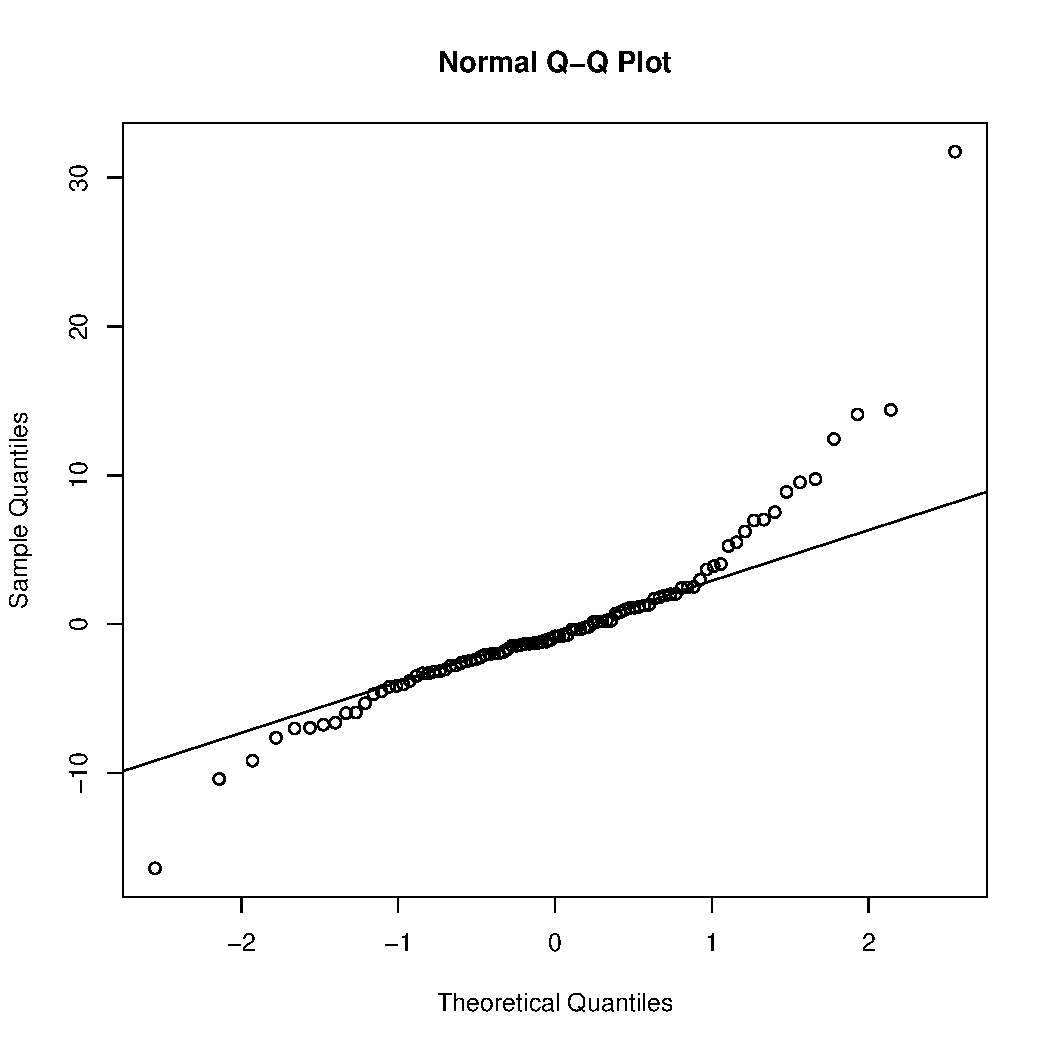
\includegraphics[width=\maxwidth]{figure/unnamed-chunk-23-1} 

}



\end{knitrout}

    \end{column}
  \end{columns}
  
\end{frame}

\watermarkon %-----------------------------------------------------------------%

\begin{frame}[allowframebreaks]{Evaluating Normality}
  
  Next to Q-Q Plots, one of the simplest ways to evaluate the normality of the 
  error distribution is through the \emph{skewness} and \emph{kurtosis}.
  \begin{itemize}
  \item Skewness and kurtosis are functions of the third and fourth moments, 
    respectively.
  \end{itemize}
  \vb
  The \emph{moments} of a distribution are single number summaries of the 
  distribution's characteristics.
  \begin{itemize}
  \item The zeroth moment is the total probability mass.
  \item The first moment is the mean.
  \item The second central moment is the variance.
  \item The third standardized moment is the skewness.
  \item The fourth standardized moment is the kurtosis.
  \end{itemize}
  
\end{frame}

%------------------------------------------------------------------------------%

\begin{frame}{Moments}
  
  The $k$th raw moment of $X$ (around zero):
  \begin{align*}
    M_k = \text{E}\left[X^k\right]
  \end{align*}
  The $k$th central moment of $X$:
  \begin{align*}
    \widetilde{M}_k = \text{E}\left[(X - \text{E}[X])^k\right] = \text{E}\left[(X - \mu)^k\right]
  \end{align*}
  The $k$th standardized moment of $X$:
  \begin{align*}
    M_k^* &= \frac{\text{E}\left[(X - \text{E}[X])^k\right]}{\left(\sqrt{\text{E}\left[(X - \text{E}[X])^2\right]}\right)^k} = \frac{\text{E}\left[(X - \mu_1)^k\right]}{\sigma^k}
  \end{align*}
  
\end{frame}

%------------------------------------------------------------------------------%

\begin{frame}{Skewness}
  
  The skewness, $\gamma$, is the third standardized moment of $X$.
  \begin{align*}
    \gamma = M_3^* = \frac{E\left[(X - \mu)^3\right]}{\sigma^3}
  \end{align*}
  Skewness tells us about asymmetry in the distribution.
  \begin{itemize}
  \item The normal distribution has skewness $\gamma = 0$.
  \item Positively skewed distributions (i.e., $\gamma > 0$) will have long 
    right tails.
  \item Negatively skewed distributions (i.e., $\gamma < 0$) will have long left 
    tails.
  \end{itemize}
  \vb
  A common cutoff says that skewness with a magnitude greater than 1 (i.e., 
  $|\gamma| > 1$) indicates substantial non-normality.
  
\end{frame}

\watermarkoff %----------------------------------------------------------------%

\begin{frame}{Skewed Distributions}
  
  \begin{columns}
    \begin{column}{0.5\textwidth}
  
\begin{knitrout}\footnotesize
\definecolor{shadecolor}{rgb}{0.878, 0.918, 0.933}\color{fgcolor}

{\centering 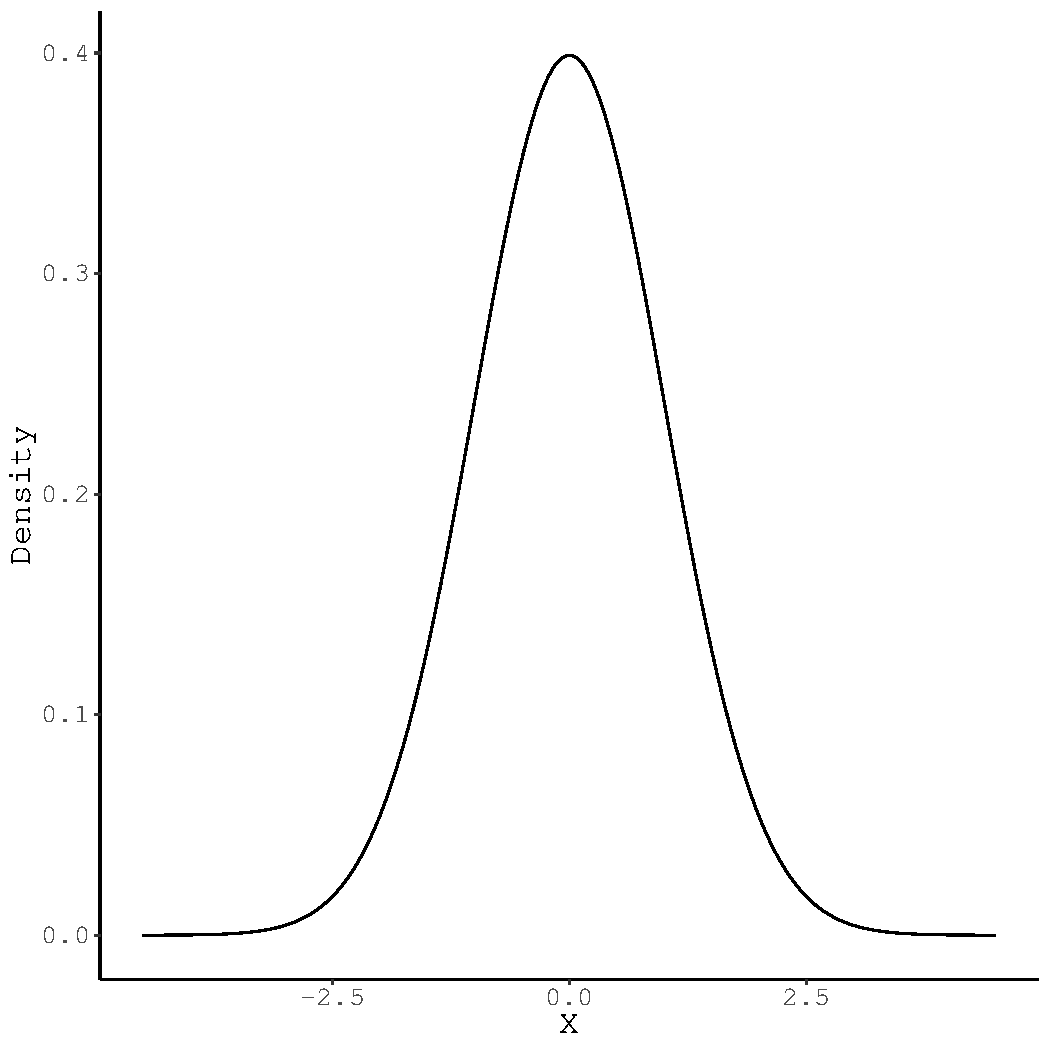
\includegraphics[width=\maxwidth]{figure/unnamed-chunk-24-1} 

}



\end{knitrout}

    \end{column}
    
    \begin{column}{0.5\textwidth}
        
\begin{knitrout}\footnotesize
\definecolor{shadecolor}{rgb}{0.878, 0.918, 0.933}\color{fgcolor}

{\centering 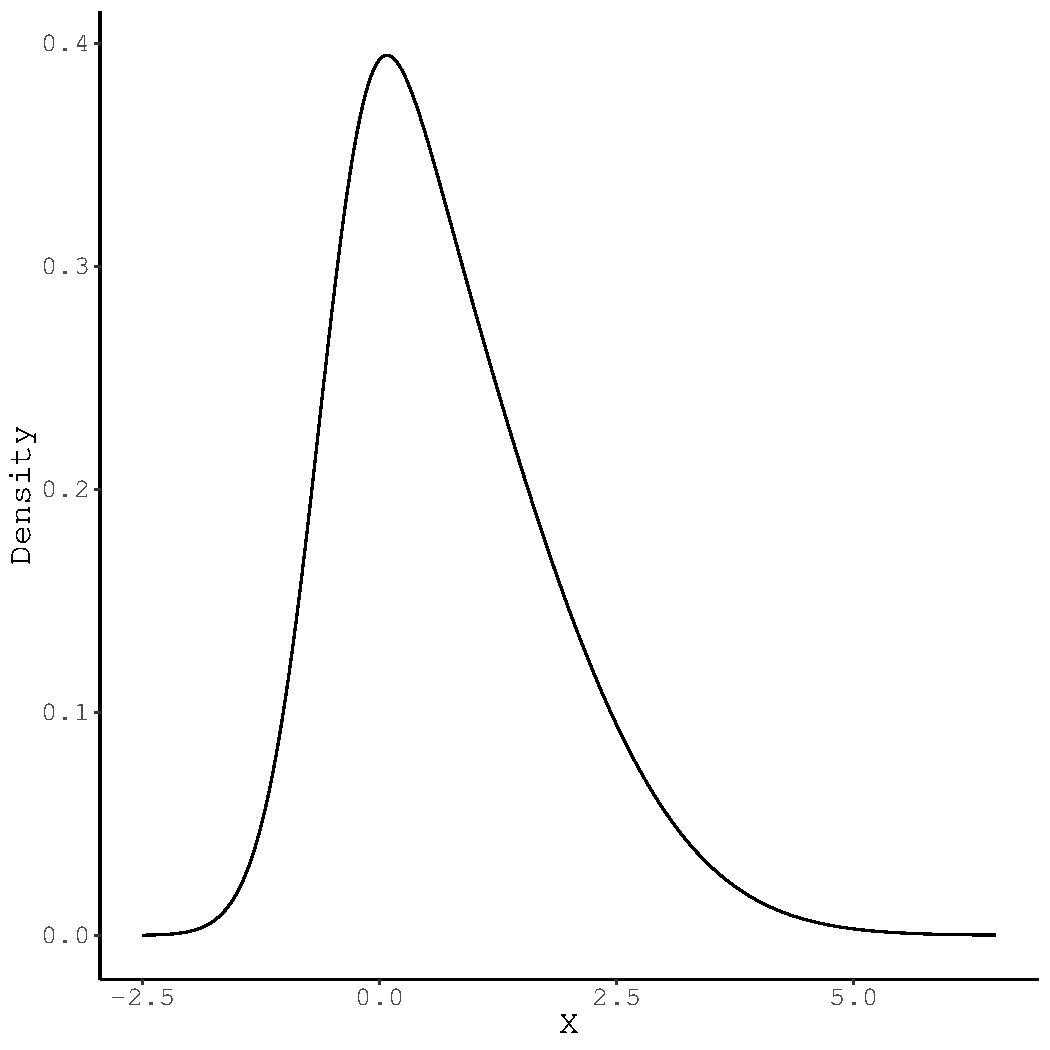
\includegraphics[width=0.6\linewidth]{figure/unnamed-chunk-25-1} 

}




{\centering 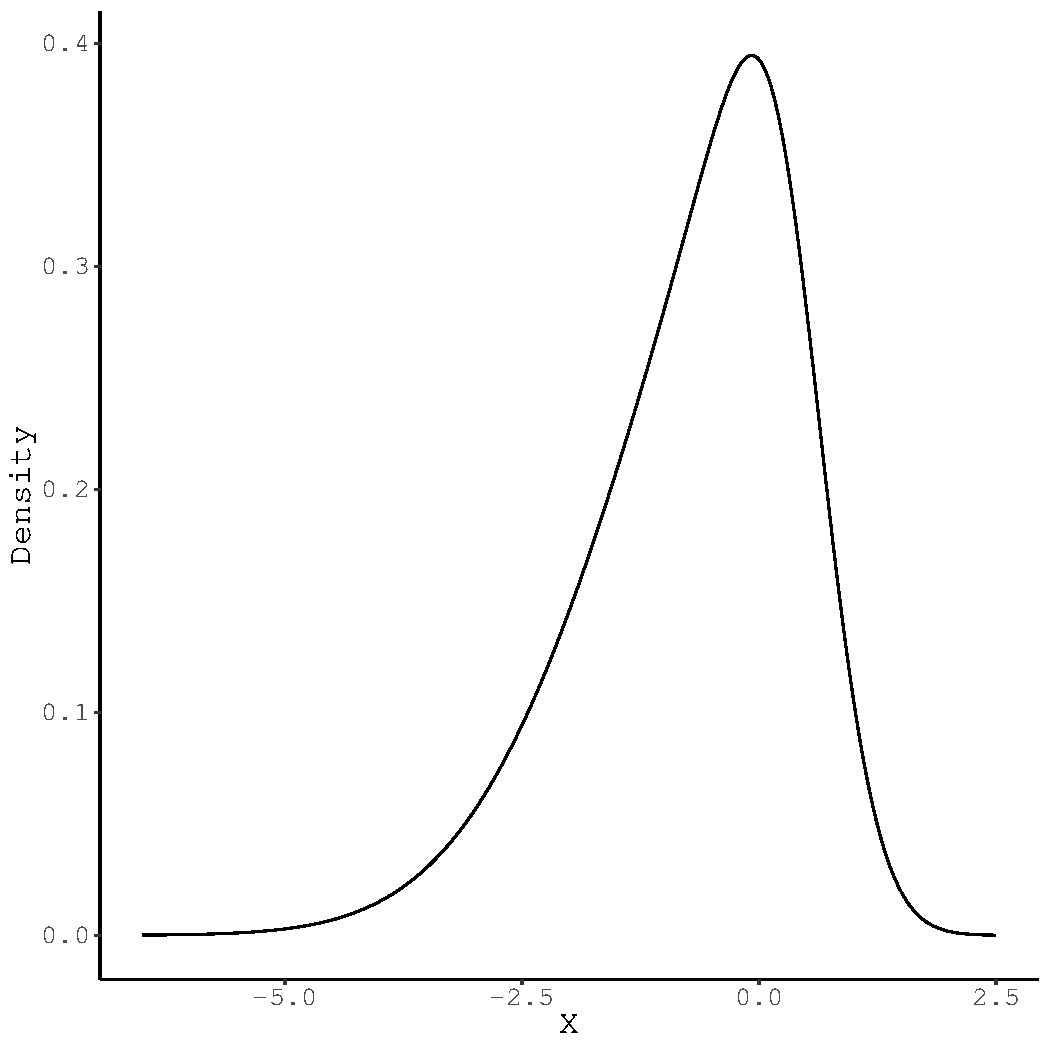
\includegraphics[width=0.6\linewidth]{figure/unnamed-chunk-25-2} 

}



\end{knitrout}

\end{column}
\end{columns}
  
\end{frame}

\watermarkon %-----------------------------------------------------------------%

\begin{frame}{Kurtosis}
  
  The kurtosis, $\kappa_0$, is the fourth standardized moment of $X$.
  \begin{align*}
    \kappa_0 = M_4^* = \frac{E\left[(X - \mu)^4\right]}{\sigma^4}
  \end{align*}
  Kurtosis tells us about the relative heaviness of the distribution's tails.
  \begin{itemize}
  \item The normal distribution has a raw kurtosis of $\kappa_0 = 3$.
  \item The \emph{excess kurtosis}, $\kappa = \kappa_0 - 3$, is a more common 
    measure.
  \item Positive excess kurtosis indicates heavy tails.
  \item Negative excess kurtosis indicates light tails.
  \end{itemize}
  \vb 
  A common cutoff says that excess kurtosis greater than 7 (i.e., 
  $\kappa_0 > 10$) indicates substantial non-normality.
  
\end{frame}

\watermarkoff %----------------------------------------------------------------%

\begin{frame}{Kurtotic Distributions}
  
  \begin{columns}
    \begin{column}{0.5\textwidth}
  
\begin{knitrout}\footnotesize
\definecolor{shadecolor}{rgb}{0.878, 0.918, 0.933}\color{fgcolor}

{\centering 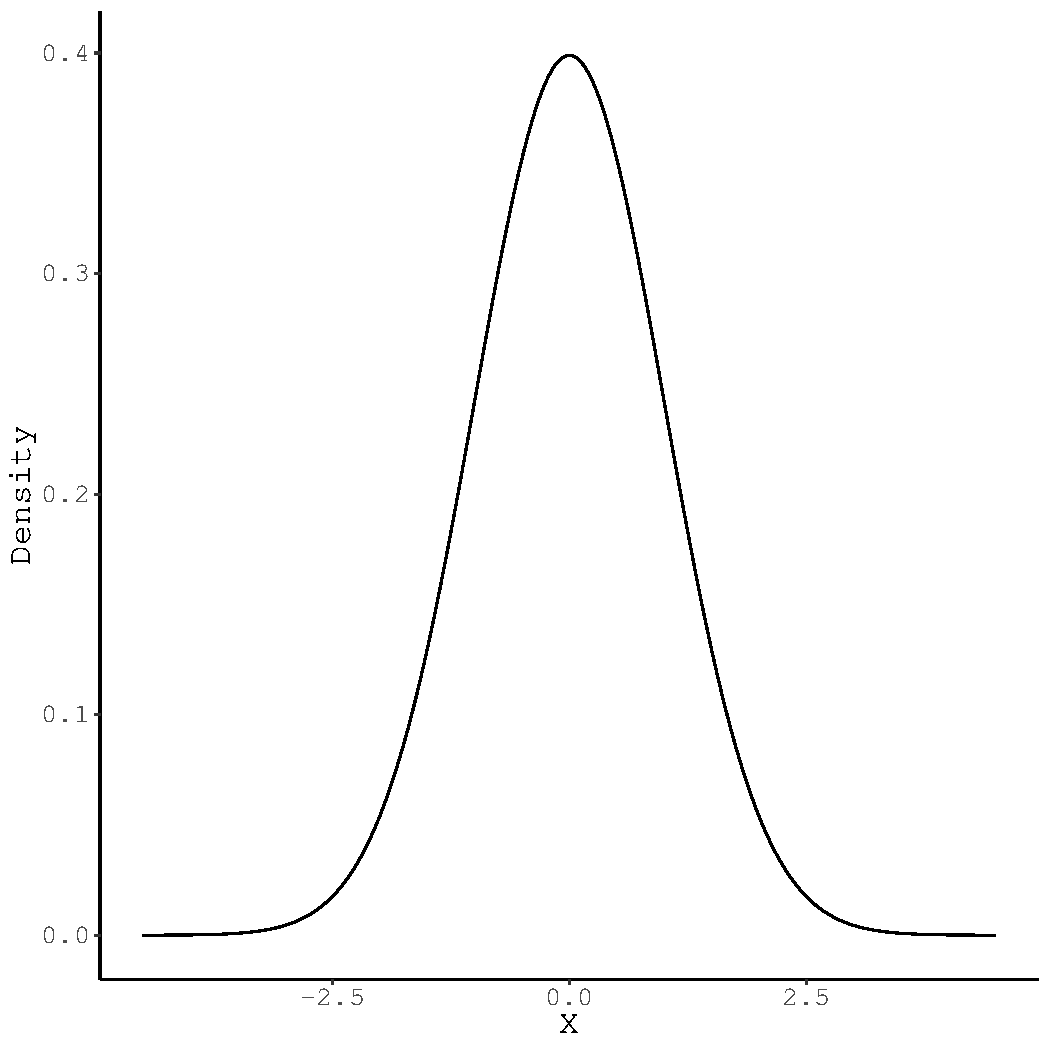
\includegraphics[width=\maxwidth]{figure/unnamed-chunk-26-1} 

}



\end{knitrout}

    \end{column}
    
    \begin{column}{0.5\textwidth}
        
\begin{knitrout}\footnotesize
\definecolor{shadecolor}{rgb}{0.878, 0.918, 0.933}\color{fgcolor}

{\centering 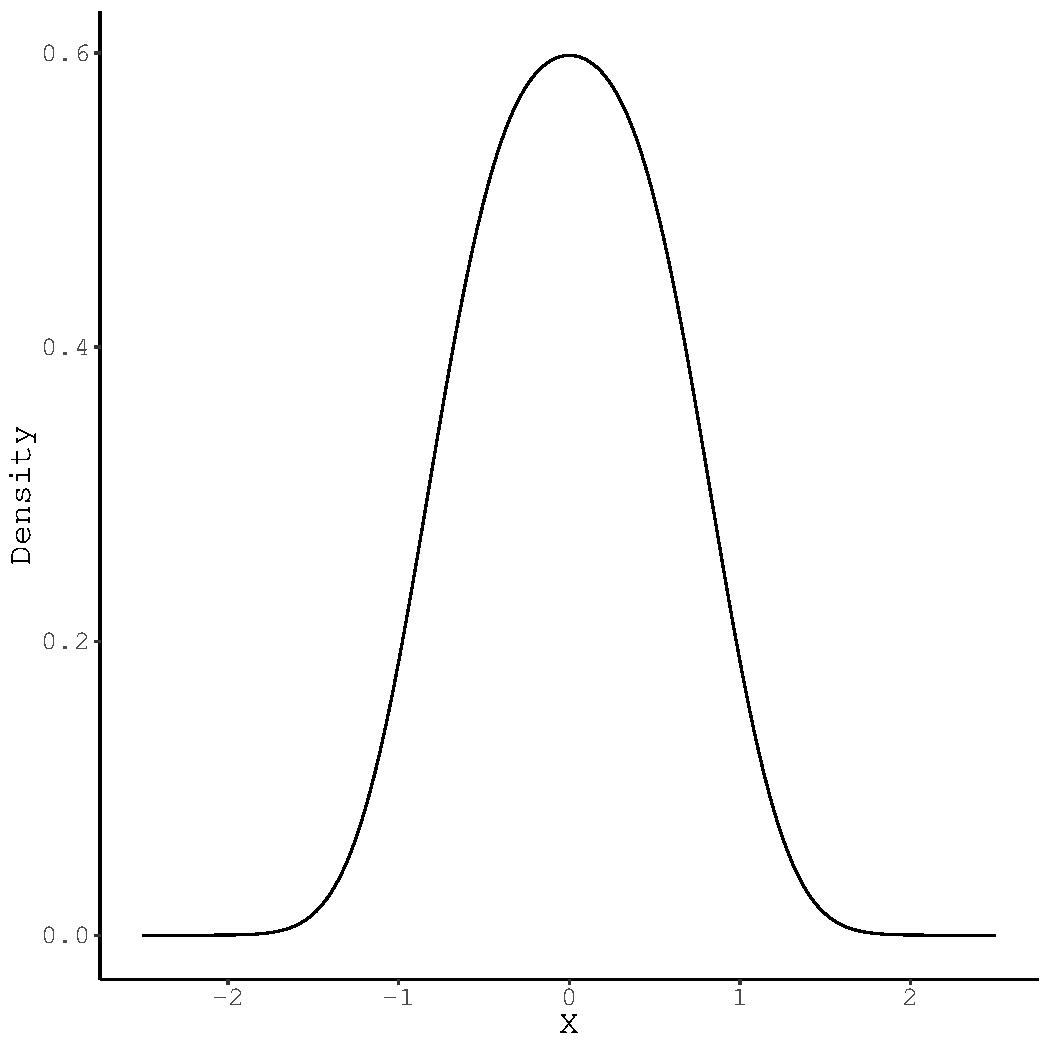
\includegraphics[width=0.6\linewidth]{figure/unnamed-chunk-27-1} 

}




{\centering 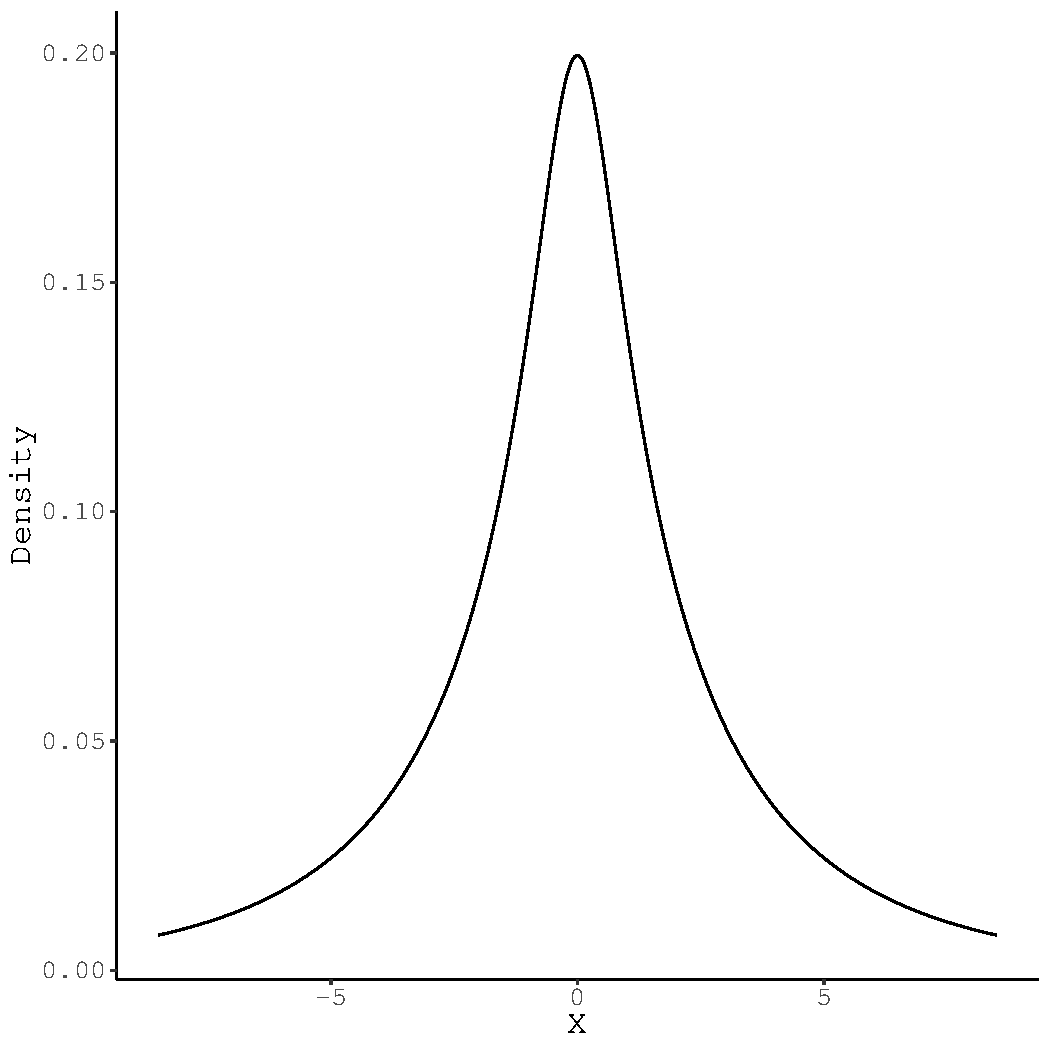
\includegraphics[width=0.6\linewidth]{figure/unnamed-chunk-27-2} 

}



\end{knitrout}

\end{column}
\end{columns}
  
\end{frame}

\watermarkon %-----------------------------------------------------------------%

\begin{frame}{Tests of Normality}
  
  We can also conduct formal statistical tests of the normality assumption.
  
  \begin{itemize}
  \item Shapiro-Wilks test
  \item Kolmogorov-Smirnov test / Lilliefors test
  \item Cramer-von Mises test
  \item Anderson-Darling test
  \end{itemize}
  
  \va
  
  These tests tend to be sensitive to sample size.
  \begin{itemize}
  \item The Shapiro-Wilks test will have the best power in small samples.
  \item The Kolmogorov-Smirnov test is probably best for large samples.
  \end{itemize}
  
\end{frame}

%------------------------------------------------------------------------------%

\begin{frame}{Consequences of Violating Normality}

  In small samples, with \emph{\underline{fixed}} predictors, normally
  distributed errors imply normal sampling distributions for the regression
  coefficients.  
  \vc
  \begin{itemize}
  \item In small samples, with \emph{\underline{random}} predictors, normal
    errors \emph{\underline{do not}} imply normally distributed coefficients.
    \vc
  \item In large samples, the central limit theorem implies normal sampling
    distributions for the coefficients, regardless of the error distribution.
  \end{itemize}
  \va
  \pause
  Prediction intervals require normally distributed errors.
  \vc
  \begin{itemize}
  \item Confidence intervals for predictions share the same normality
    requirements as the coefficients' sampling distributions.
  \end{itemize}
  
\end{frame}

%------------------------------------------------------------------------------%

\begin{frame}{Central Limit Theorem}
  
  Let $\mathcal{Z} = \{z_1, z_2, \ldots, z_N\}$ be a set of $i.i.d.$ random
  variables with mean $\mu_Z$ and (finite) standard deviation $\sigma_Z$.\\
  \begin{itemize}
  \item Define the mean of $\mathcal{Z}$ as:
    \begin{align*}
      \bar{Z} \equiv N^{-1}\sum_{n = 1}^N z_n
    \end{align*}
  \item The distribution of $\bar{Z}$ tends towards normality as $N$ increases:
    \begin{align*}
      P(\bar{Z}) \rightarrow \text{N}\left(\mu_Z, \frac{\sigma_Z}{\sqrt{N}}\right)
    \end{align*}
  \end{itemize}
  
\end{frame}

%------------------------------------------------------------------------------%

\begin{frame}{Lindeberg-Feller CLT}
  
  The Lindeberg-Feller CLT relaxes the requirement for $i.i.d.$ variables.
  \vc
  \begin{itemize}
  \item Let $\mathcal{Z} = \{z_1, z_2, \ldots, z_N\}$ be a set of
    \emph{\underline{independent}} random variables.
    \vc
    \begin{itemize}
    \item Every $z_n$ has finite variance
      \vc
    \item No $z_n$ has an overwhelmingly large variance
    \end{itemize}
    \vc
  \item The distribution of $\bar{Z}$ approaches normality as $N$ increases.
  \end{itemize}
  \va 
  \pause
  The Lindeberg-Feller CLT implies normal sampling distributions for the
  regression coefficients and predicted values in linear regression models.
  
\end{frame}

%------------------------------------------------------------------------------%

%\hat{\beta}_p &= \frac{\sum_{n = 1}^N \left(X_n -
%  \bar{X}\right)\left(Y_n - \bar{Y}\right)}{\sum_{n = 1}^N
%  \left(X_n - \bar{X}\right)^2}\\[8pt]

\begin{frame}{Central Limit Theorem for Regression}
 
  Recall the definition of our regression coefficients:
  \vx{-6}
  \begin{align*}
    \hat{\beta}_p &= \left[\textstyle{\sum_{n = 1}^N} \left(X_n - \bar{X}\right)\left(Y_n - \bar{Y}\right) \right] \text{\LARGE $\mathbin{/}$} \textstyle{\sum_{n = 1}^N} \left(X_n - \bar{X}\right)^2\\
    \hat{\beta} &= (\mathbf{X}^T\mathbf{X})^{-1}\mathbf{X}^TY = \mathbf{A}Y
  \end{align*}
  \vx{-18}
  \begin{itemize}
  \item $\mathbf{A} = (\mathbf{X}^T\mathbf{X})^{-1}\mathbf{X}^T$ is a $P \times 
    N$ matrix of
    weights.
  \end{itemize}
  \vc
  \pause
  Each of the $P$ regression coefficient can be estimated as:
  \begin{align*}
    \hat{\beta}_p &= \textstyle{\sum_{n = 1}^N} a_{pn}y_n
  \end{align*}
  \vx{-18}
  \begin{itemize}
  \item $a_{pn}$ represents the element in position $(p,n)$ of $\mathbf{A}$
  \end{itemize}
  \vc
  \pause
  If we take $a_{pn} \equiv z_n \in \mathcal{Z}$, the Lindeberg-Feller CLT
  implies normal sampling distributions for the $\hat{\beta}_p$, if $N$ is large
  enough.
  
\end{frame}
  
%------------------------------------------------------------------------------%

\begin{frame}{Central Limit Theorem for Regression}
    
  The same logic implies normal distributions for predicted values.
  \begin{align*}
    \hat{Y} &= \mathbf{X}\hat{\beta}\\
    &=\mathbf{X}(\mathbf{X}^T\mathbf{X})^{-1}\mathbf{X}^TY\\
    &=\mathbf{H}Y
  \end{align*}
  \vx{-24}
  \begin{itemize}
  \item $\mathbf{H}$ is an $N \times N$ projection matrix (the \emph{hat}
    matrix).
  \end{itemize}
  \vb
  \pause
  Each of the $N$ predicted values can be estimated as:
  \begin{align*}
    \hat{Y}_n = \sum_{i = 1}^N h_{ni}y_i
  \end{align*}
  \vx{-12}
  \begin{itemize}
  \item $h_{ni}$ represents the element in position $(n, i)$ of $\mathbf{H}$.
  \end{itemize}
  
\end{frame}

%------------------------------------------------------------------------------%

\begin{frame}{Treating Violations of Normality}
  
  We usually don't need to do anything about non-normal errors.
  \begin{itemize}
  \item The CLT will protect our inferences.
  \end{itemize}
  \vb 
  \pause
  We can use \emph{bootstrapping} to get around the need for normality.
  \begin{enumerate}
  \item Treat your sample as a synthetic population from which you draw many new
    samples (with replacement).
  \item Estimate your model in each new sample.
  \item The replicates of your estimated parameters generate an empirical
    sampling distribution that you can use for inference.
  \end{enumerate}
  \vb
  \pause
  Bootstrapping can be used for inference on pretty much any estimable
  parameter, but it won't work with small samples.
  \begin{itemize}
  \item Need to assume that your sample is representative of the population
  \end{itemize}
  
\end{frame}

%------------------------------------------------------------------------------%

\begin{frame}{Influential Observations}
  
  Influential observations contaminate analyses in two ways:
  \vc
  \begin{enumerate}
  \item Exert too much influence on the fitted regression model
    \vc
  \item Invalidate estimates/inferences by violating assumptions
  \end{enumerate}
  \vb
  There are two distinct types of influential observations:
  \vc
  \begin{enumerate}
  \item Outliers
    \vc
    \begin{itemize}
    \item Observations with extreme outcome values, relative to the other data.
      \vc
    \item Observations with outcome values that fit the model very badly.
    \end{itemize}
    \vb
  \item High-leverage observations
    \vc
    \begin{itemize}
    \item Observation with extreme predictor values, relative to other data.
    \end{itemize}
  \end{enumerate}
  
\end{frame}
    
%------------------------------------------------------------------------------%

\begin{frame}{Outliers}
  
  Outliers can be identified by scrutinizing the residuals.
  \vc
  \begin{itemize}
  \item Observations with residuals of large magnitude may be outliers.
    \vc
  \item The difficulty arises in quantifying what constitutes a ``large'' 
    residual.
  \end{itemize}
  \vb 
  If the residuals do not have constant variance, then we cannot directly 
  compare them.
  \vc
  \begin{itemize}
  \item We need to standardize the residuals in some way.
  \end{itemize}
  
\end{frame}

%------------------------------------------------------------------------------%

\begin{frame}{Detecting Outliers}
  
  We are specifically interested in \emph{externally studentized residuals}.
  \vb
  \begin{itemize}
  \item We can't simply standardize the ordinary residuals.
    \begin{itemize}
    \item \emph{Internally studentized residuals}
      \vc
    \item Outliers can pull the regression line towards themselves.
      \vc
    \item The internally studentized residuals for outliers will be too small.
    \end{itemize}
  \end{itemize}
  \vb
  Begin by defining the concept of a \emph{deleted residual}:
  \begin{align*}
    \hat{\varepsilon}_{(n)} = Y_n - \hat{Y}_{(n)}
  \end{align*}
  \vx{-18}
  \begin{itemize}
    \item $\hat{\varepsilon}_{(n)}$ quantifies the distance of $Y_n$ from the 
      regression line estimated after excluding the $n$th observation.
  \end{itemize}
  
\end{frame}

%------------------------------------------------------------------------------%

\begin{frame}{Studentized Residuals}
  
  If we standardize the deleted residual, $\hat{\varepsilon}_{(n)}$, we get the 
  externally studentized residual:
  \begin{align*}
    t_{(n)} = \frac{\hat{\varepsilon}_{(n)}}{SE_{\hat{\varepsilon}_{(n)}}}
  \end{align*}
  The externally studentized residuals have two very useful properties:
  \vb
  \begin{enumerate}
  \item Each $t_{(n)}$ is scaled equivalently.
    \vc
    \begin{itemize}
    \item We can directly compare different $t_{(n)}$.
    \end{itemize}
    \vb
  \item The $t_{(n)}$ are \emph{Student's t} distributed.
    \vc
    \begin{itemize}
    \item We can quantify outliers in terms of quantiles of the $t$
      distribution.
      \vc
    \item $|t_{(n)}| > 3.0$ is a common rule of thumb for flagging outliers.
    \end{itemize}
  \end{enumerate}
  
\end{frame}

\watermarkoff %----------------------------------------------------------------%

\begin{frame}{Studentized Residual Plots}
  
  \begin{columns}
    \begin{column}{0.5\textwidth}
      
      Index plots of the externally studentized residuals can help spotlight 
      potential outliers.
      \vb
      \begin{itemize}
      \item Look for observations that clearly ``stand out from the crowd.''
      \end{itemize}
      
    \end{column}
    
    \begin{column}{0.5\textwidth}
\begin{knitrout}\footnotesize
\definecolor{shadecolor}{rgb}{0.878, 0.918, 0.933}\color{fgcolor}

{\centering 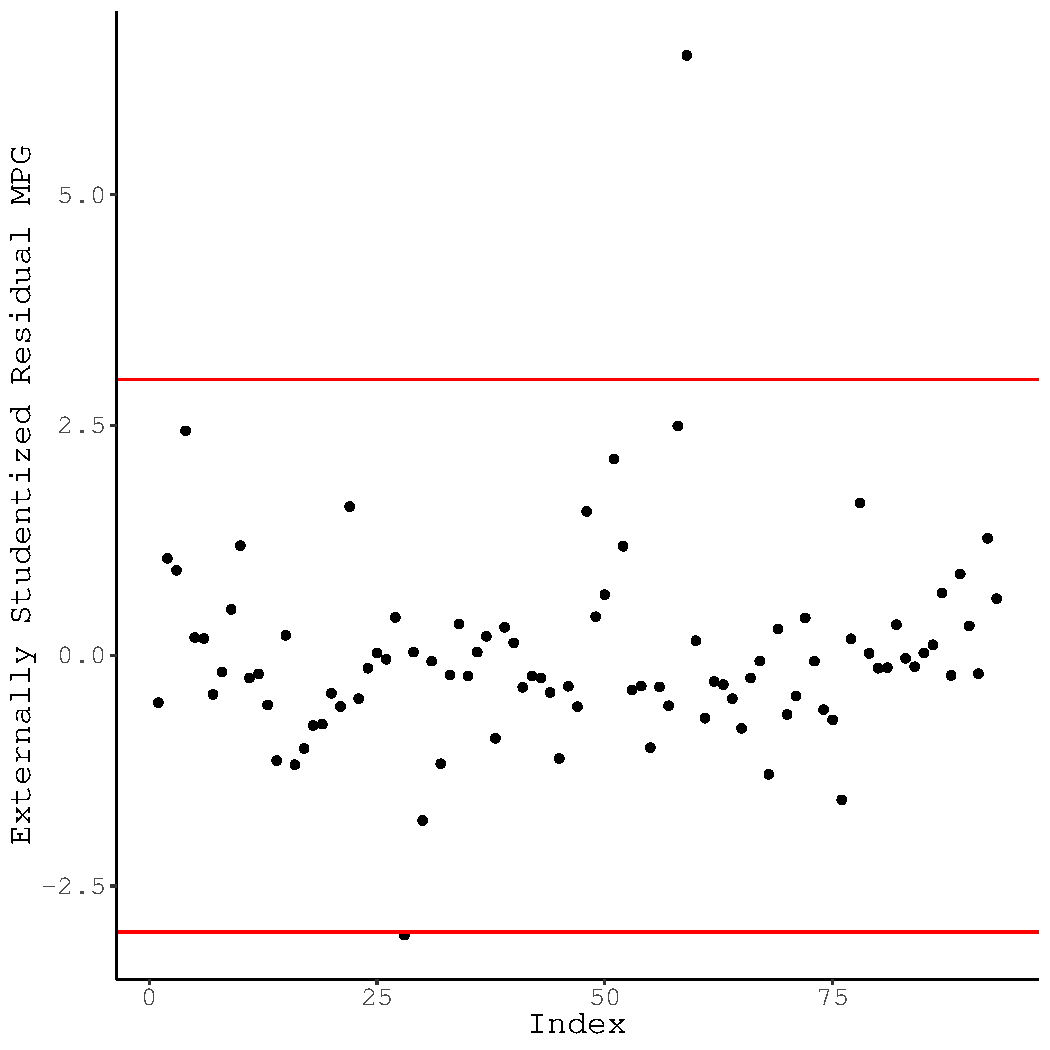
\includegraphics[width=\maxwidth]{figure/unnamed-chunk-28-1} 

}



\end{knitrout}

\end{column}
\end{columns}

\end{frame}

%------------------------------------------------------------------------------%

\begin{frame}{High-Leverage Points}
  
  We identify high-leverage observations through their \emph{leverage} values.
  \vb
  \begin{itemize}
  \item An observation's leverage, $h_n$, quantifies the extent to which its
    predictors affect the fitted regression model.  
    \vb
  \item Observations with $X$ values very far from the mean, $\bar{X}$, affect
    the fitted model disproportionately.  
  \end{itemize}
  \vb
  \pause
  In simple linear regression, the $n$th leverage is given by:
  \begin{align*}
    h_n = \frac{1}{N} + \frac{\left(X_n - \bar{X}\right)^2}
    {\sum_{m = 1}^N \left(X_{m} - \bar{X}\right)^2}
  \end{align*}\\
  \pause
  In multiple linear regression, the leverages are given by the diagonal of the 
  hat matrix, $\mathbf{H} = \mathbf{X}(\mathbf{X}^T\mathbf{X})^{-1}\mathbf{X}^T$:
  \begin{align*}
    h_n &= \mathbf{H}[n, n]
  \end{align*}
  
\end{frame}

%------------------------------------------------------------------------------%

\begin{frame}{Properties of Leverages}
  
  Leverages have the following useful properties:
  \vb
  \begin{itemize}
  \item $h_n$ grows in direct proportion to the distance between $X_n$ and
    $\bar{X}$.  
    \vb
  \item $h_n \in \left[\frac{1}{N}, 1.0\right]$
    \vb
  \item $\bar{h} = \frac{P + 1}{N}$
  \end{itemize}
  \vb
  Observations with $h_n \gg \bar{h}$ are potentially influential.
  
\end{frame}

\watermarkoff %----------------------------------------------------------------%

\begin{frame}{Leverage Plots}
  
  \begin{columns}
    \begin{column}{0.5\textwidth}
      
      Index plots of the leverage values can help spotlight high-leverage points.
      \vb
      \begin{itemize}
      \item Again, look for observations that clearly ``stand out from the 
        crowd.''
      \end{itemize}
      
    \end{column}
    
    \begin{column}{0.5\textwidth}
\begin{knitrout}\footnotesize
\definecolor{shadecolor}{rgb}{0.878, 0.918, 0.933}\color{fgcolor}

{\centering 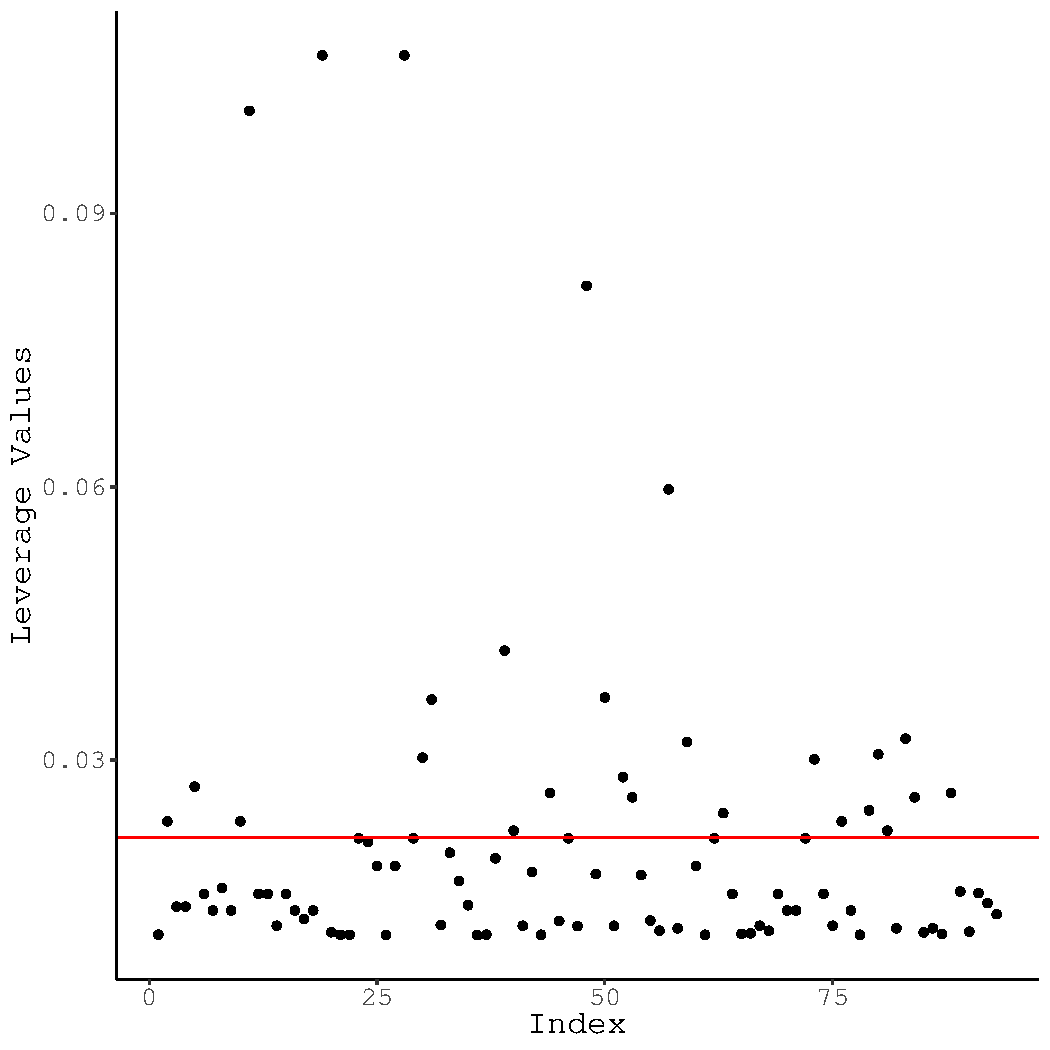
\includegraphics[width=\maxwidth]{figure/unnamed-chunk-29-1} 

}



\end{knitrout}

\end{column}
\end{columns}

\end{frame}

\watermarkon %-----------------------------------------------------------------%
    
\begin{frame}{From Outliers and Leverages to Influential Points}
  
  Observations with high leverage or large (externally) studentized residuals
  are not necessarily influential.
  \vc
  \begin{itemize}
  \item High-leverage observations tend to be more influential than outliers.
    \vc
  \item The worst problems arise from observations that are both outliers and
    have high leverage.
  \end{itemize}
  \vb 
  \emph{Measures of influence} simultaneously consider extremity in both $X$
  and $Y$ dimensions.
  \vc
  \begin{itemize}
  \item Observations with high measures of influence are very likely to cause
    problems.
  \end{itemize}
  
\end{frame}

%------------------------------------------------------------------------------%

\begin{frame}{Measures of Influence}
  
  Measures of influence come in two flavors:
  \vb
  \begin{enumerate}
  \item Global measures of influence
    \begin{itemize}
    \item Cook's $D$
      \vc
    \item$\textit{DFFITS}$
    \end{itemize}
    \vb
  \item Coefficient-specific measures of influence
    \vb
    \begin{itemize}
    \item $\textit{DFBETAS}$
    \end{itemize}
  \end{enumerate}
  \vb
  All measures of influence use the same logic as the deleted residual.
  \vc
  \begin{itemize}
  \item Compare models estimated from the whole sample to models estimated from 
    samples excluding individual observations.
  \end{itemize}
\end{frame}

%------------------------------------------------------------------------------%

\begin{frame}{Global Measures of Influence}
  
  Cook's $D$ and $\textit{DFFITS}$ are more-or-less interchangeable measures.
  \vb
  \begin{itemize}
  \item They each provide very similar information.
    \vb
  \item They will tend to lead to the same conclusions.
  \end{itemize}
  \begin{align*}
    \textit{DFFITS}_n &= \frac{\hat{Y}_n - \hat{Y}_{(n)}}{\sqrt{\hat{\sigma}^2_{(n)} h_n}} = t_{(n)} \sqrt{\frac{h_n}{1 - h_n}}\\[8pt]
    \text{Cook's} ~ D_n &= \frac{\sum_{n = 1}^N \left( \hat{Y}_n - \hat{Y}_{(n)} \right)^2}{\left(P + 1\right) \hat{\sigma}^2} = (P + 1)^{-1} t_n^2 \frac{h_n}{1 - h_n}
  \end{align*}
  
\end{frame}

%------------------------------------------------------------------------------%

\begin{frame}{Rules-of-Thumb}
  
  The recommend thresholds for problematic degrees of global influence: 
  \vb
  \begin{itemize}
  \item $|\textit{DFFITS}_n| > 2\sqrt{\frac{P + 1}{N}}$
    \vb
  \item Cook's $D_n >$ the critical $F$ value for $\alpha = 0.5$, $df_{num} =
    P + 1$, and $df_{den} = N - P - 1$
  \end{itemize}
  
\end{frame}

\watermarkoff %----------------------------------------------------------------%

\begin{frame}{Plots of Global Measures of Influence}
  
  \begin{columns}
    \begin{column}{0.5\textwidth}
      
\begin{knitrout}\footnotesize
\definecolor{shadecolor}{rgb}{0.878, 0.918, 0.933}\color{fgcolor}

{\centering 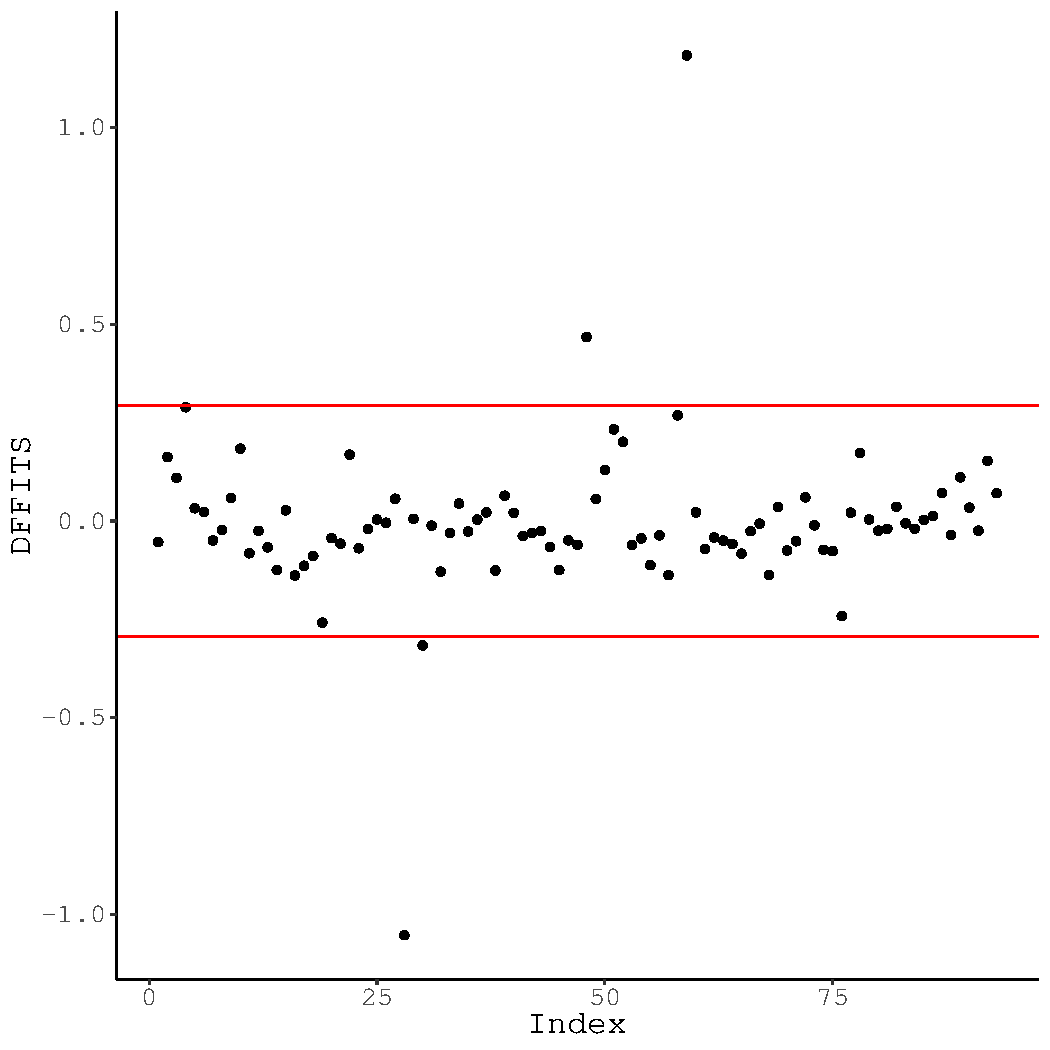
\includegraphics[width=\maxwidth]{figure/unnamed-chunk-30-1} 

}



\end{knitrout}

\end{column}
    
    \begin{column}{0.5\textwidth}

\begin{knitrout}\footnotesize
\definecolor{shadecolor}{rgb}{0.878, 0.918, 0.933}\color{fgcolor}

{\centering 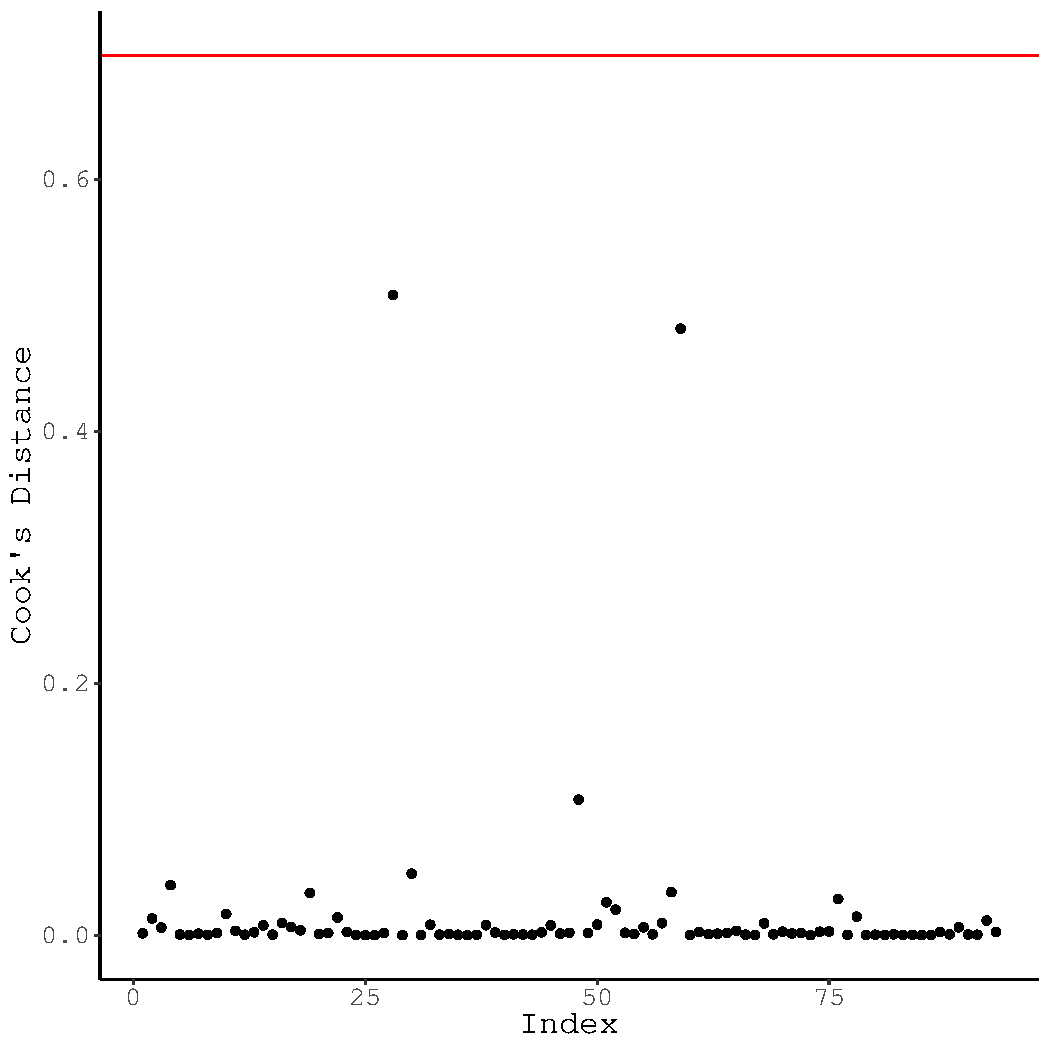
\includegraphics[width=\maxwidth]{figure/unnamed-chunk-31-1} 

}



\end{knitrout}

\end{column}
\end{columns}

\end{frame}

\watermarkon %-----------------------------------------------------------------%

\begin{frame}{Coefficient-Specific Measures of Influence}
  
  Each regression coefficient (including the intercept) gets a \emph{DFBETAS}
  value for each observation.
  \begin{align*}
    \textit{DFBETAS}_{np} = \frac{\hat{\beta}_p - \hat{\beta}_{p(n)}}
           {\textit{SE}_{\hat{\beta}_{p(n)}}}
  \end{align*}
  The rule-of-thumb for flagging influential observations:
  \vb
  \begin{itemize}
  \item $|\textit{DFBETAS}_{np}| > \frac{2}{\sqrt{N}}$
  \end{itemize}
  
\end{frame}

\watermarkoff %----------------------------------------------------------------%

\begin{frame}{Plots of Coefficient-Specific Measures}
  
  \begin{columns}
    \begin{column}{0.5\textwidth}
      
\begin{knitrout}\footnotesize
\definecolor{shadecolor}{rgb}{0.878, 0.918, 0.933}\color{fgcolor}

{\centering 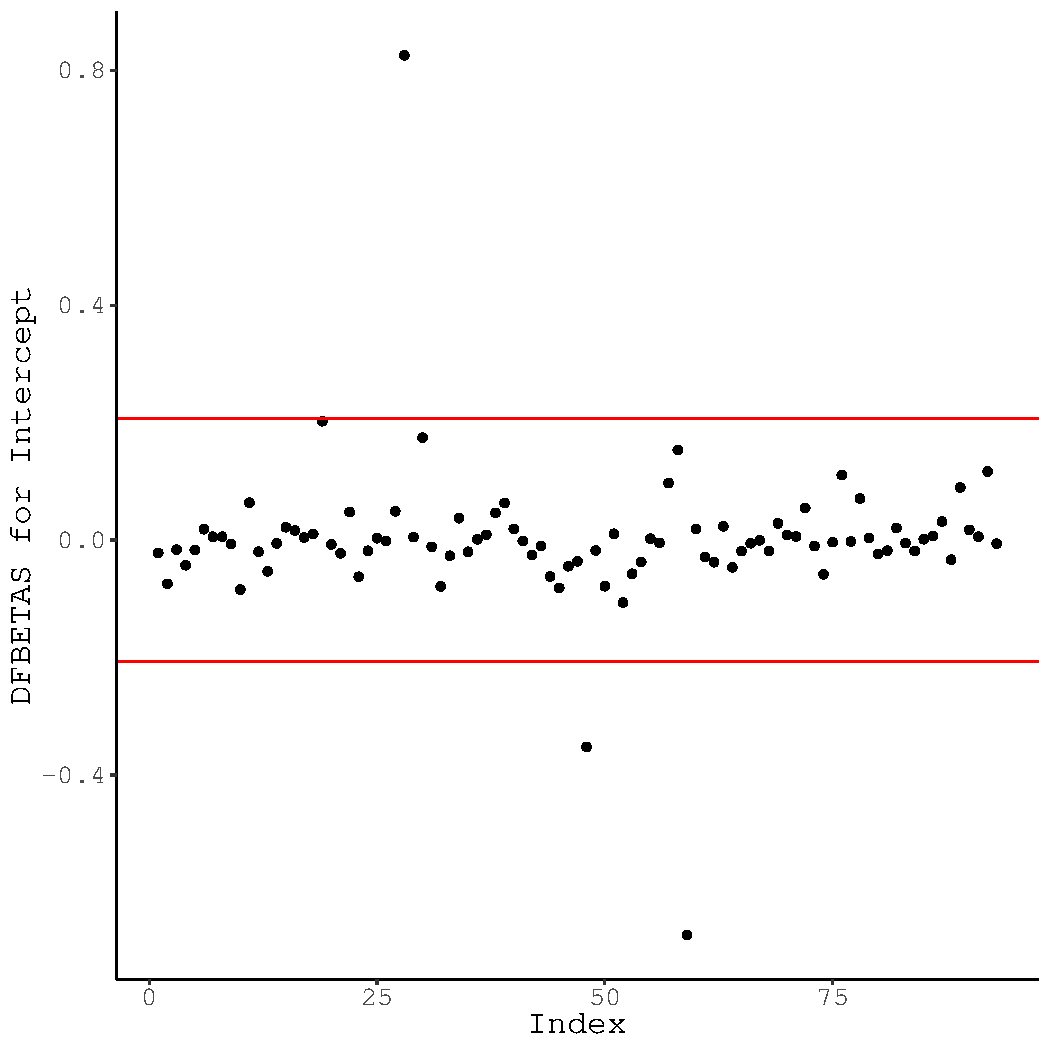
\includegraphics[width=\maxwidth]{figure/unnamed-chunk-32-1} 

}



\end{knitrout}

\end{column}
    
    \begin{column}{0.5\textwidth}

\begin{knitrout}\footnotesize
\definecolor{shadecolor}{rgb}{0.878, 0.918, 0.933}\color{fgcolor}

{\centering 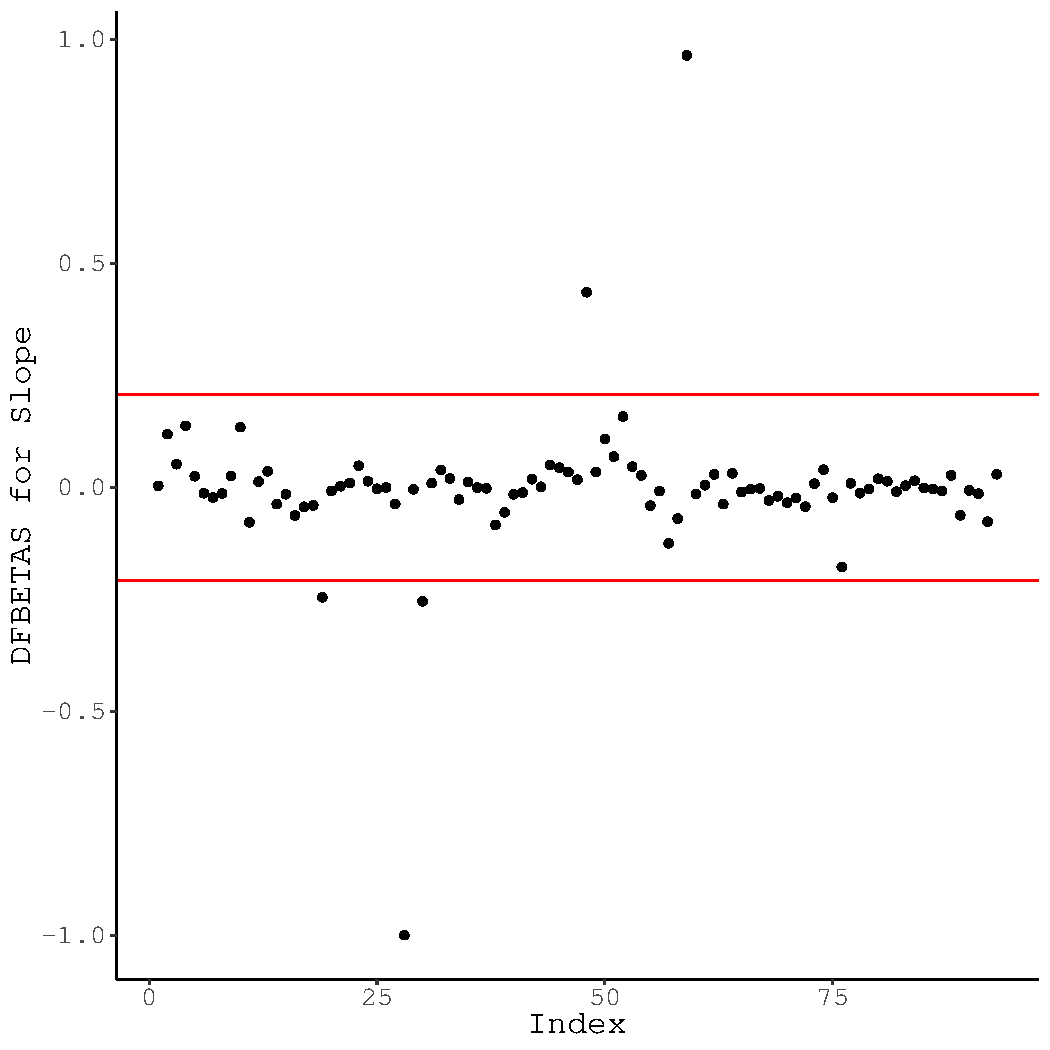
\includegraphics[width=\maxwidth]{figure/unnamed-chunk-33-1} 

}



\end{knitrout}

\end{column}
\end{columns}

\end{frame}

%------------------------------------------------------------------------------%

\begin{frame}{Consequences of Removing Influential Observations}
    
  \begin{columns}
    \begin{column}{0.5\textwidth}
      
      Observation number 59 was the most influential according to \emph{DFFITS}.
      \vb
      \begin{itemize}
      \item Removing that observation has a small impact on the fitted 
        regression line.  
        \vc
      \item Influential observations don't only affect the regression line, 
        though.
      \end{itemize}
      
    \end{column}
    
    \begin{column}{0.5\textwidth}
      
\begin{knitrout}\footnotesize
\definecolor{shadecolor}{rgb}{0.878, 0.918, 0.933}\color{fgcolor}

{\centering 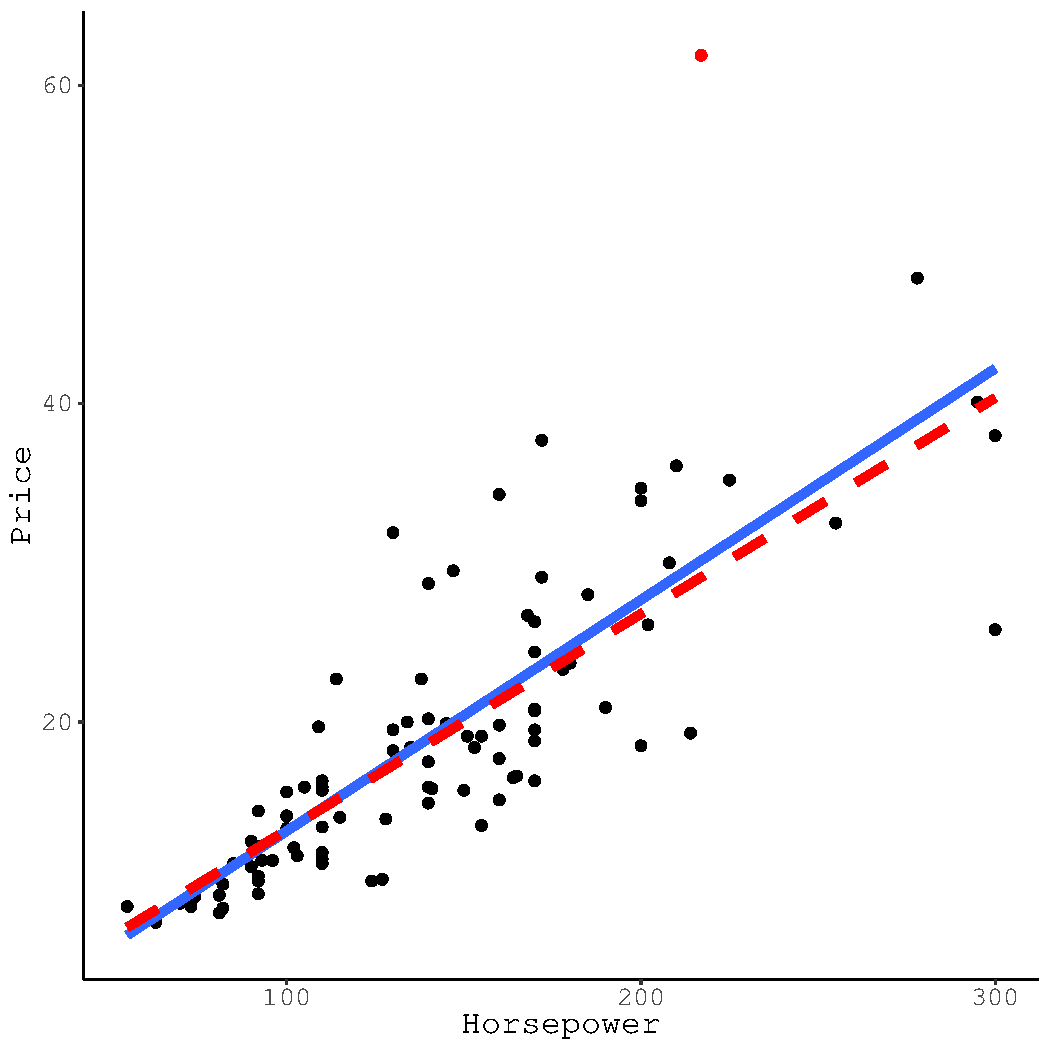
\includegraphics[width=\maxwidth]{figure/unnamed-chunk-34-1} 

}



\end{knitrout}

\end{column}
\end{columns}

\end{frame}

%------------------------------------------------------------------------------%

\begin{frame}[fragile, allowframebreaks]{Consequences of Removing Influential 
    Observations}
  
\begin{knitrout}\footnotesize
\definecolor{shadecolor}{rgb}{0.878, 0.918, 0.933}\color{fgcolor}\begin{kframe}
\begin{alltt}
\hlcom{## Fit model with full sample:}
\hlstd{out1} \hlkwb{<-} \hlkwd{lm}\hlstd{(Price} \hlopt{~} \hlstd{Horsepower,} \hlkwc{data} \hlstd{= Cars93)}

\hlcom{## Exclude outliers:}
\hlstd{Cars93.2} \hlkwb{<-} \hlstd{Cars93[}\hlopt{-}\hlnum{59}\hlstd{, ]}

\hlcom{## Fit model with reduced sample:}
\hlstd{out2} \hlkwb{<-} \hlkwd{lm}\hlstd{(Price} \hlopt{~} \hlstd{Horsepower,} \hlkwc{data} \hlstd{= Cars93.2)}
\end{alltt}
\end{kframe}
\end{knitrout}

\pagebreak

\begin{knitrout}\footnotesize
\definecolor{shadecolor}{rgb}{0.878, 0.918, 0.933}\color{fgcolor}\begin{kframe}
\begin{alltt}
\hlkwd{round}\hlstd{(}\hlkwd{summary}\hlstd{(out1)}\hlopt{$}\hlstd{coefficients,} \hlnum{6}\hlstd{)}
\end{alltt}
\begin{verbatim}
##              Estimate Std. Error   t value Pr(>|t|)
## (Intercept) -1.398769   1.820016 -0.768548 0.444152
## Horsepower   0.145371   0.011898 12.218325 0.000000
\end{verbatim}
\begin{alltt}
\hlkwd{round}\hlstd{(}\hlkwd{summary}\hlstd{(out2)}\hlopt{$}\hlstd{coefficients,} \hlnum{6}\hlstd{)}
\end{alltt}
\begin{verbatim}
##              Estimate Std. Error   t value Pr(>|t|)
## (Intercept) -0.383557    1.51673 -0.252884 0.800934
## Horsepower   0.135860    0.00997 13.626694 0.000000
\end{verbatim}
\end{kframe}
\end{knitrout}

\pagebreak

\begin{knitrout}\footnotesize
\definecolor{shadecolor}{rgb}{0.878, 0.918, 0.933}\color{fgcolor}\begin{kframe}
\begin{alltt}
\hlkwd{partSummary}\hlstd{(out1,} \hlnum{2}\hlstd{)}
\end{alltt}
\begin{verbatim}
## Residuals:
##     Min      1Q  Median      3Q     Max 
## -16.413  -2.792  -0.821   1.803  31.753
\end{verbatim}
\begin{alltt}
\hlkwd{partSummary}\hlstd{(out2,} \hlnum{2}\hlstd{)}
\end{alltt}
\begin{verbatim}
## Residuals:
##      Min       1Q   Median       3Q      Max 
## -14.5746  -2.6501  -0.9477   1.8087  14.7156
\end{verbatim}
\end{kframe}
\end{knitrout}

\pagebreak

\begin{knitrout}\footnotesize
\definecolor{shadecolor}{rgb}{0.878, 0.918, 0.933}\color{fgcolor}\begin{kframe}
\begin{alltt}
\hlkwd{unlist}\hlstd{(}
    \hlkwd{summary}\hlstd{(out1)[}\hlkwd{c}\hlstd{(}\hlstr{"sigma"}\hlstd{,} \hlstr{"r.squared"}\hlstd{,} \hlstr{"fstatistic"}\hlstd{)]}
\hlstd{)[}\hlnum{1} \hlopt{:} \hlnum{3}\hlstd{]}
\end{alltt}
\begin{verbatim}
##            sigma        r.squared fstatistic.value 
##         5.976953         0.621287       149.287468
\end{verbatim}
\begin{alltt}
\hlkwd{unlist}\hlstd{(}
    \hlkwd{summary}\hlstd{(out2)[}\hlkwd{c}\hlstd{(}\hlstr{"sigma"}\hlstd{,} \hlstr{"r.squared"}\hlstd{,} \hlstr{"fstatistic"}\hlstd{)]}
\hlstd{)[}\hlnum{1} \hlopt{:} \hlnum{3}\hlstd{]}
\end{alltt}
\begin{verbatim}
##            sigma        r.squared fstatistic.value 
##        4.9545903        0.6735426      185.6867952
\end{verbatim}
\end{kframe}
\end{knitrout}

\end{frame}

%------------------------------------------------------------------------------%

\begin{frame}{Consequences of Removing Influential Observations}
    
  \begin{columns}
    \begin{column}{0.5\textwidth}
      
      If we remove the two most influential observations, $n = \{28, 59\}$, the 
      fitted regression line barely changes at all.  
      \vc
      \begin{itemize}
      \item The influences of these two observations were counteracting one 
        another.
      \item We're probably still better off, though.
      \end{itemize}
      
    \end{column}
    
    \begin{column}{0.5\textwidth}
      
\begin{knitrout}\footnotesize
\definecolor{shadecolor}{rgb}{0.878, 0.918, 0.933}\color{fgcolor}

{\centering 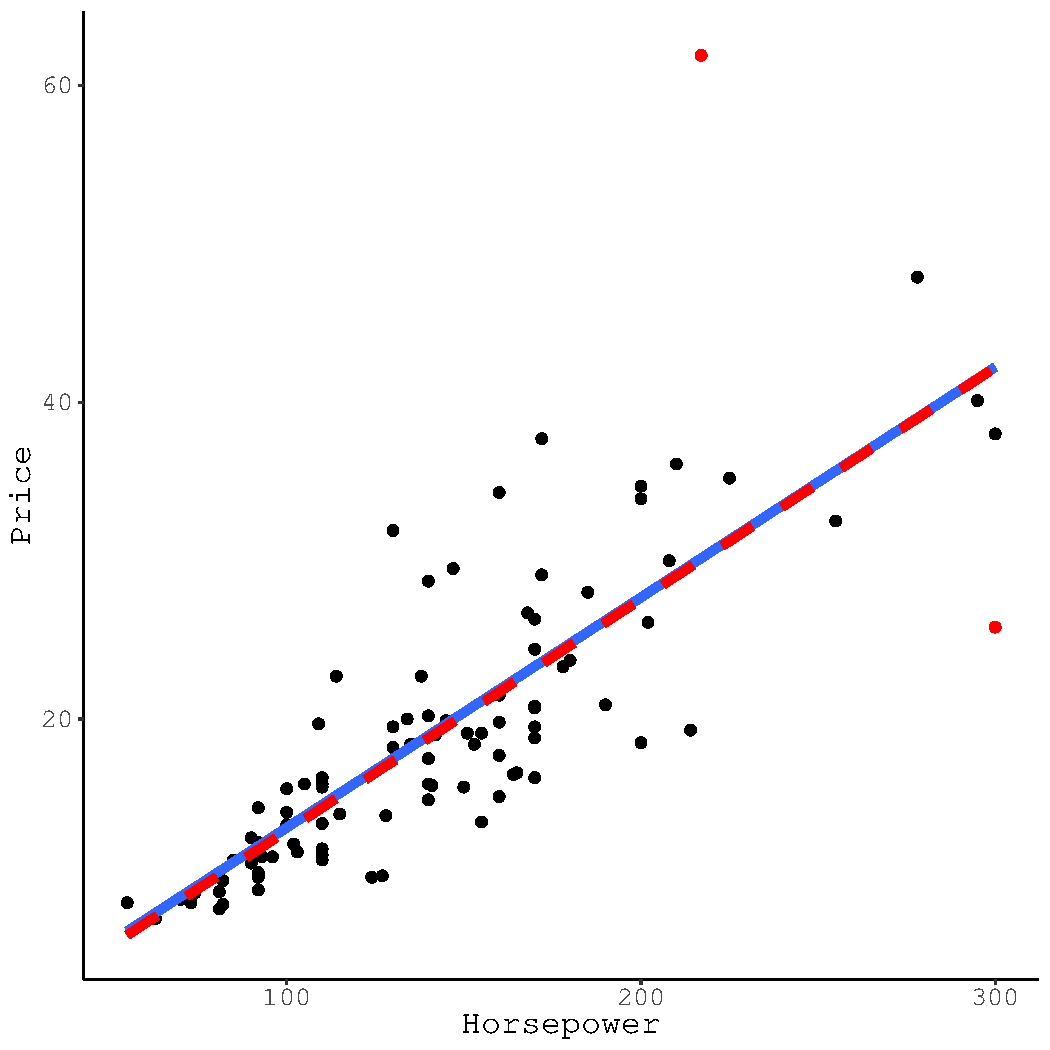
\includegraphics[width=\maxwidth]{figure/unnamed-chunk-39-1} 

}



\end{knitrout}

\end{column}
\end{columns}

\end{frame}

%------------------------------------------------------------------------------%

\begin{frame}[fragile, allowframebreaks]{Consequences of Removing Influential 
    Observations}
  
\begin{knitrout}\footnotesize
\definecolor{shadecolor}{rgb}{0.878, 0.918, 0.933}\color{fgcolor}\begin{kframe}
\begin{alltt}
\hlcom{## Fit model with full sample:}
\hlstd{out1.2} \hlkwb{<-} \hlkwd{lm}\hlstd{(Price} \hlopt{~} \hlstd{Horsepower,} \hlkwc{data} \hlstd{= Cars93)}

\hlcom{## Exclude outliers:}
\hlstd{Cars93.2} \hlkwb{<-} \hlstd{Cars93[}\hlopt{-}\hlkwd{c}\hlstd{(}\hlnum{28}\hlstd{,} \hlnum{59}\hlstd{), ]}

\hlcom{## Fit model with reduced sample:}
\hlstd{out2.2} \hlkwb{<-} \hlkwd{lm}\hlstd{(Price} \hlopt{~} \hlstd{Horsepower,} \hlkwc{data} \hlstd{= Cars93.2)}
\end{alltt}
\end{kframe}
\end{knitrout}

\pagebreak

\begin{knitrout}\footnotesize
\definecolor{shadecolor}{rgb}{0.878, 0.918, 0.933}\color{fgcolor}\begin{kframe}
\begin{alltt}
\hlkwd{round}\hlstd{(}\hlkwd{summary}\hlstd{(out1.2)}\hlopt{$}\hlstd{coefficients,} \hlnum{6}\hlstd{)}
\end{alltt}
\begin{verbatim}
##              Estimate Std. Error   t value Pr(>|t|)
## (Intercept) -1.398769   1.820016 -0.768548 0.444152
## Horsepower   0.145371   0.011898 12.218325 0.000000
\end{verbatim}
\begin{alltt}
\hlkwd{round}\hlstd{(}\hlkwd{summary}\hlstd{(out2.2)}\hlopt{$}\hlstd{coefficients,} \hlnum{6}\hlstd{)}
\end{alltt}
\begin{verbatim}
##              Estimate Std. Error   t value Pr(>|t|)
## (Intercept) -1.695315   1.494767 -1.134166  0.25977
## Horsepower   0.146277   0.009986 14.648807  0.00000
\end{verbatim}
\end{kframe}
\end{knitrout}

\pagebreak

\begin{knitrout}\footnotesize
\definecolor{shadecolor}{rgb}{0.878, 0.918, 0.933}\color{fgcolor}\begin{kframe}
\begin{alltt}
\hlkwd{partSummary}\hlstd{(out1.2,} \hlnum{2}\hlstd{)}
\end{alltt}
\begin{verbatim}
## Residuals:
##     Min      1Q  Median      3Q     Max 
## -16.413  -2.792  -0.821   1.803  31.753
\end{verbatim}
\begin{alltt}
\hlkwd{partSummary}\hlstd{(out2.2,} \hlnum{2}\hlstd{)}
\end{alltt}
\begin{verbatim}
## Residuals:
##      Min       1Q   Median       3Q      Max 
## -10.3079  -2.5786  -0.6084   1.9775  14.5793
\end{verbatim}
\end{kframe}
\end{knitrout}

\pagebreak

\begin{knitrout}\footnotesize
\definecolor{shadecolor}{rgb}{0.878, 0.918, 0.933}\color{fgcolor}\begin{kframe}
\begin{alltt}
\hlkwd{unlist}\hlstd{(}
    \hlkwd{summary}\hlstd{(out1.2)[}\hlkwd{c}\hlstd{(}\hlstr{"sigma"}\hlstd{,} \hlstr{"r.squared"}\hlstd{,} \hlstr{"fstatistic"}\hlstd{)]}
\hlstd{)[}\hlnum{1} \hlopt{:} \hlnum{3}\hlstd{]}
\end{alltt}
\begin{verbatim}
##            sigma        r.squared fstatistic.value 
##         5.976953         0.621287       149.287468
\end{verbatim}
\begin{alltt}
\hlkwd{unlist}\hlstd{(}
    \hlkwd{summary}\hlstd{(out2.2)[}\hlkwd{c}\hlstd{(}\hlstr{"sigma"}\hlstd{,} \hlstr{"r.squared"}\hlstd{,} \hlstr{"fstatistic"}\hlstd{)]}
\hlstd{)[}\hlnum{1} \hlopt{:} \hlnum{3}\hlstd{]}
\end{alltt}
\begin{verbatim}
##            sigma        r.squared fstatistic.value 
##        4.7053314        0.7068391      214.5875491
\end{verbatim}
\end{kframe}
\end{knitrout}

\end{frame}

%------------------------------------------------------------------------------%

\begin{frame}{Influential Points Violating Assumptions}
  
  \begin{columns}
    \begin{column}{0.5\textwidth}
      
      Let's revisit the nonlinear relationship between \emph{Horsepower} and
      \emph{MPG}.  \vb
      \begin{itemize}
      \item The residual plots never really behaved.
        \vc
      \item Maybe some influential observations are causing trouble?
        \vc
        \begin{itemize}
        \item $n = 39$ certainly looks like a jerk.
        \end{itemize}
      \end{itemize}
      
    \end{column}
    
    \begin{column}{0.5\textwidth}
      
\begin{knitrout}\footnotesize
\definecolor{shadecolor}{rgb}{0.878, 0.918, 0.933}\color{fgcolor}

{\centering 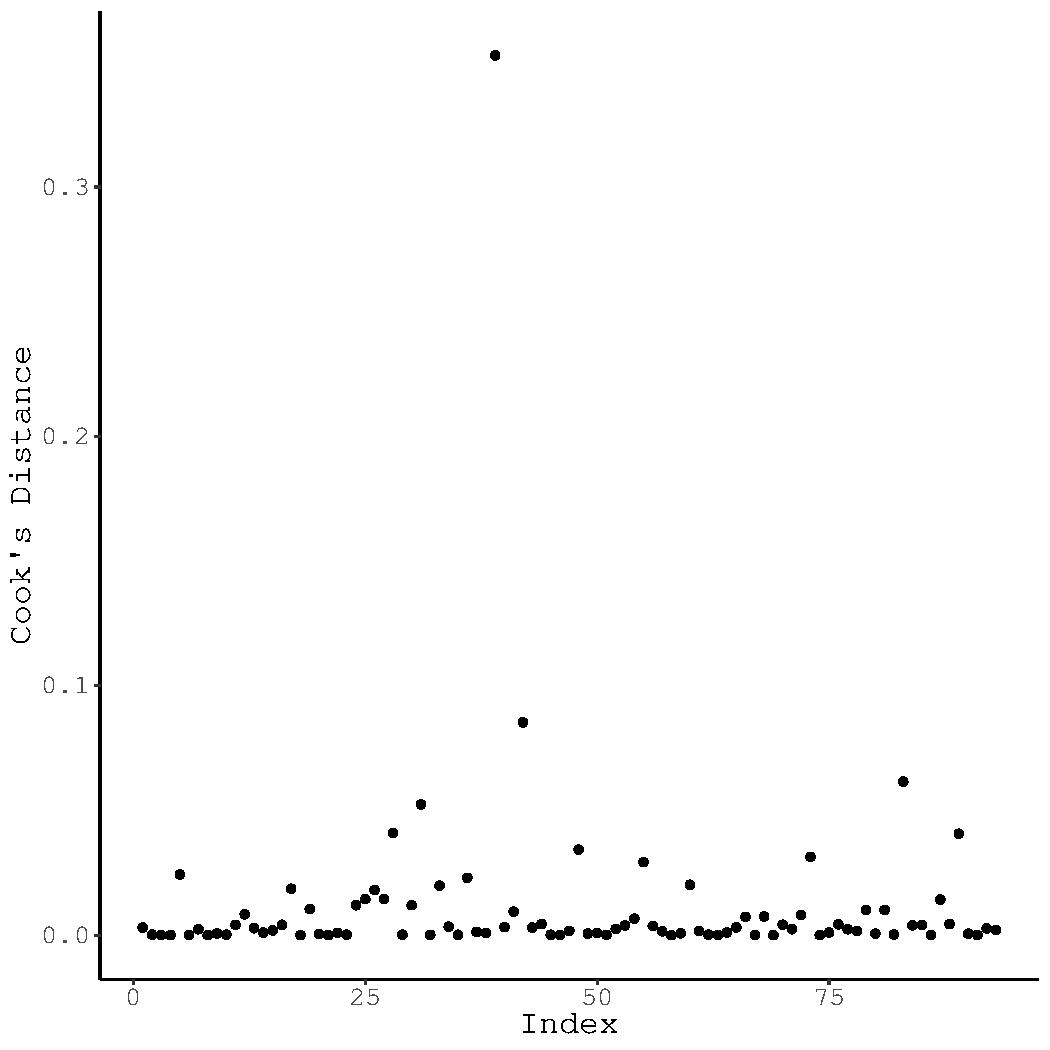
\includegraphics[width=\maxwidth]{figure/unnamed-chunk-44-1} 

}



\end{knitrout}

\end{column}
\end{columns}

\end{frame}

%------------------------------------------------------------------------------%

\begin{frame}{Quadratic Model}

  Residuals look much smoother after deleting the influential point.
  \vb
  \begin{columns}
    \begin{column}{0.5\textwidth}
      
\begin{knitrout}\footnotesize
\definecolor{shadecolor}{rgb}{0.878, 0.918, 0.933}\color{fgcolor}

{\centering 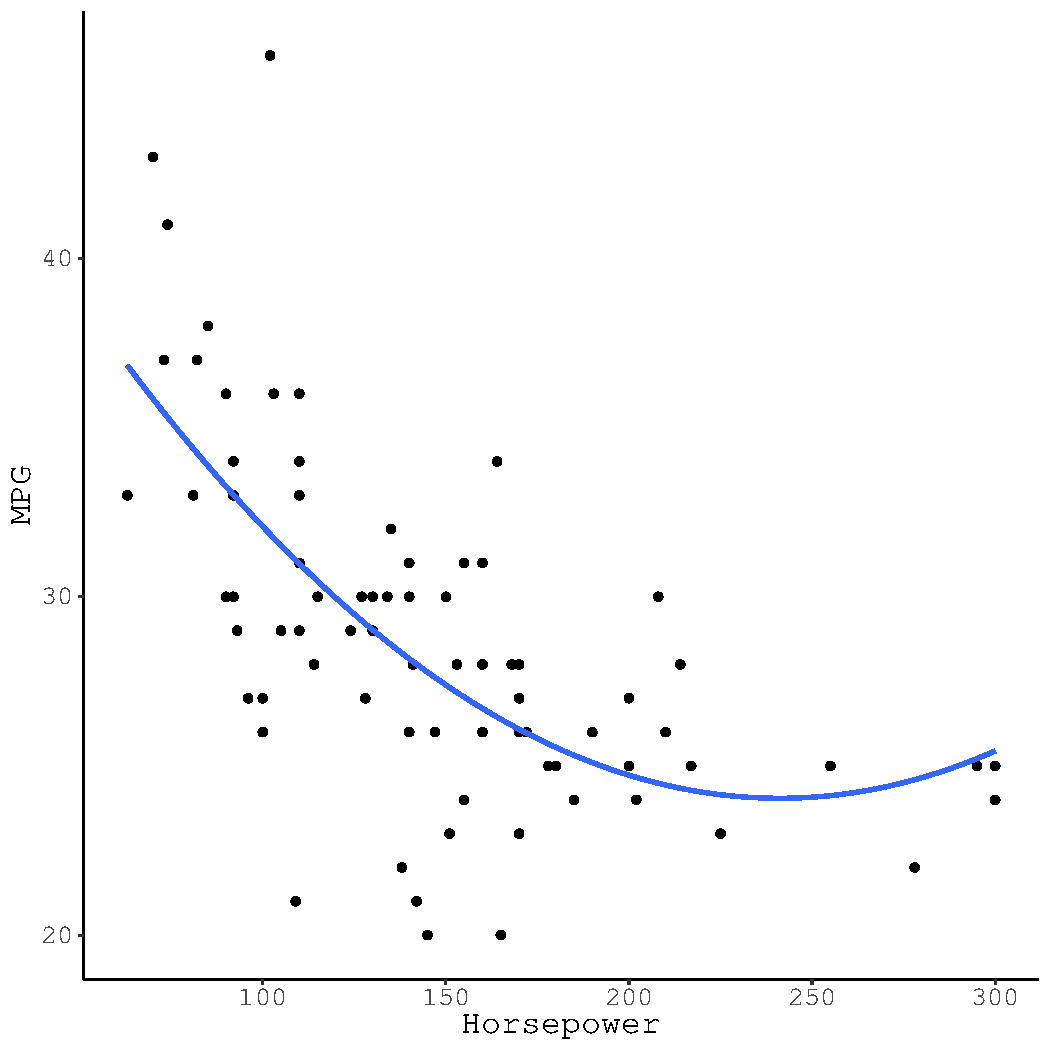
\includegraphics[width=\maxwidth]{figure/unnamed-chunk-45-1} 

}



\end{knitrout}

\end{column}

\begin{column}{0.5\textwidth}
      
\begin{knitrout}\footnotesize
\definecolor{shadecolor}{rgb}{0.878, 0.918, 0.933}\color{fgcolor}

{\centering 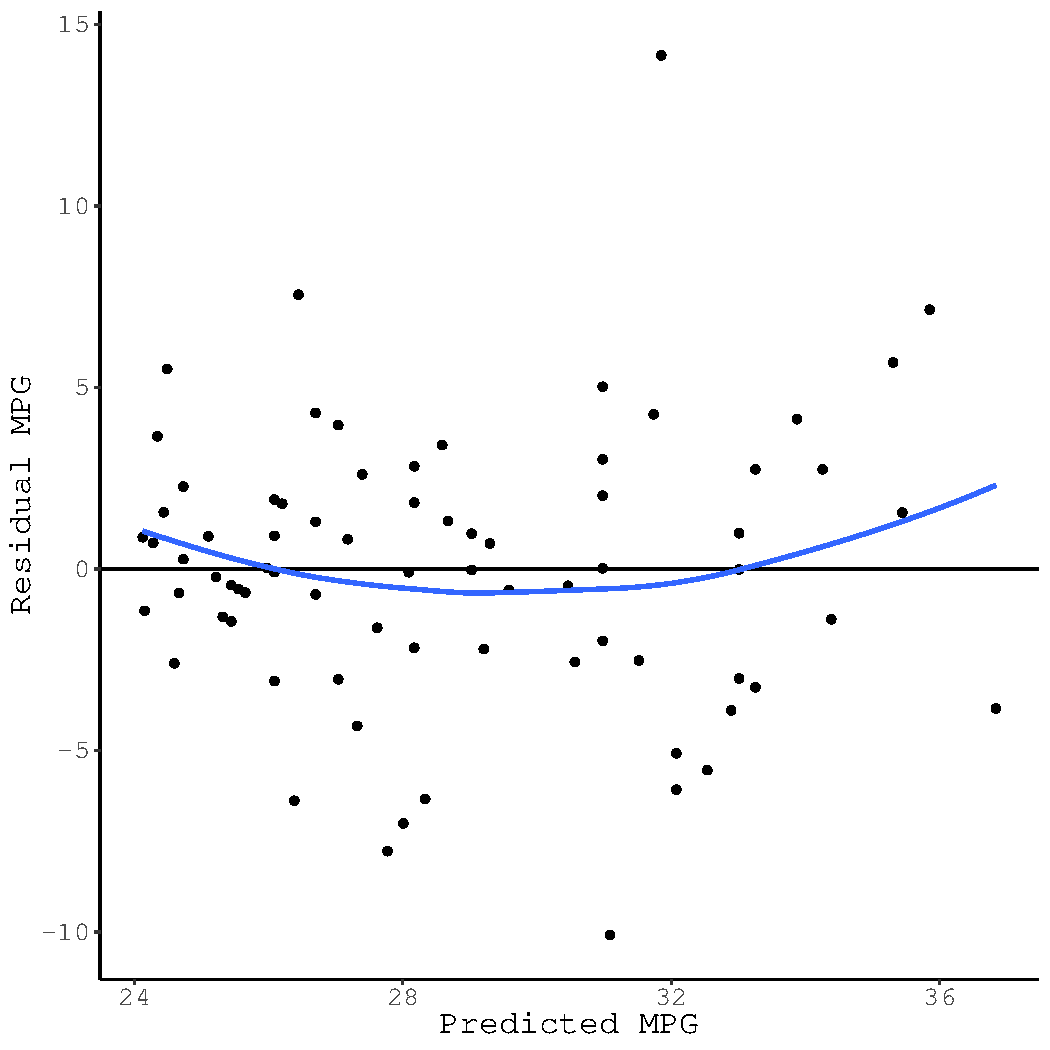
\includegraphics[width=\maxwidth]{figure/unnamed-chunk-46-1} 

}



\end{knitrout}

\end{column}
\end{columns}
  
\end{frame}

%------------------------------------------------------------------------------%

\begin{frame}{Cubic Model}

  Basically no trend, after fitting the cubic model to the reduced dataset.
  \vb
  \begin{columns}
    \begin{column}{0.5\textwidth}
      
\begin{knitrout}\footnotesize
\definecolor{shadecolor}{rgb}{0.878, 0.918, 0.933}\color{fgcolor}

{\centering 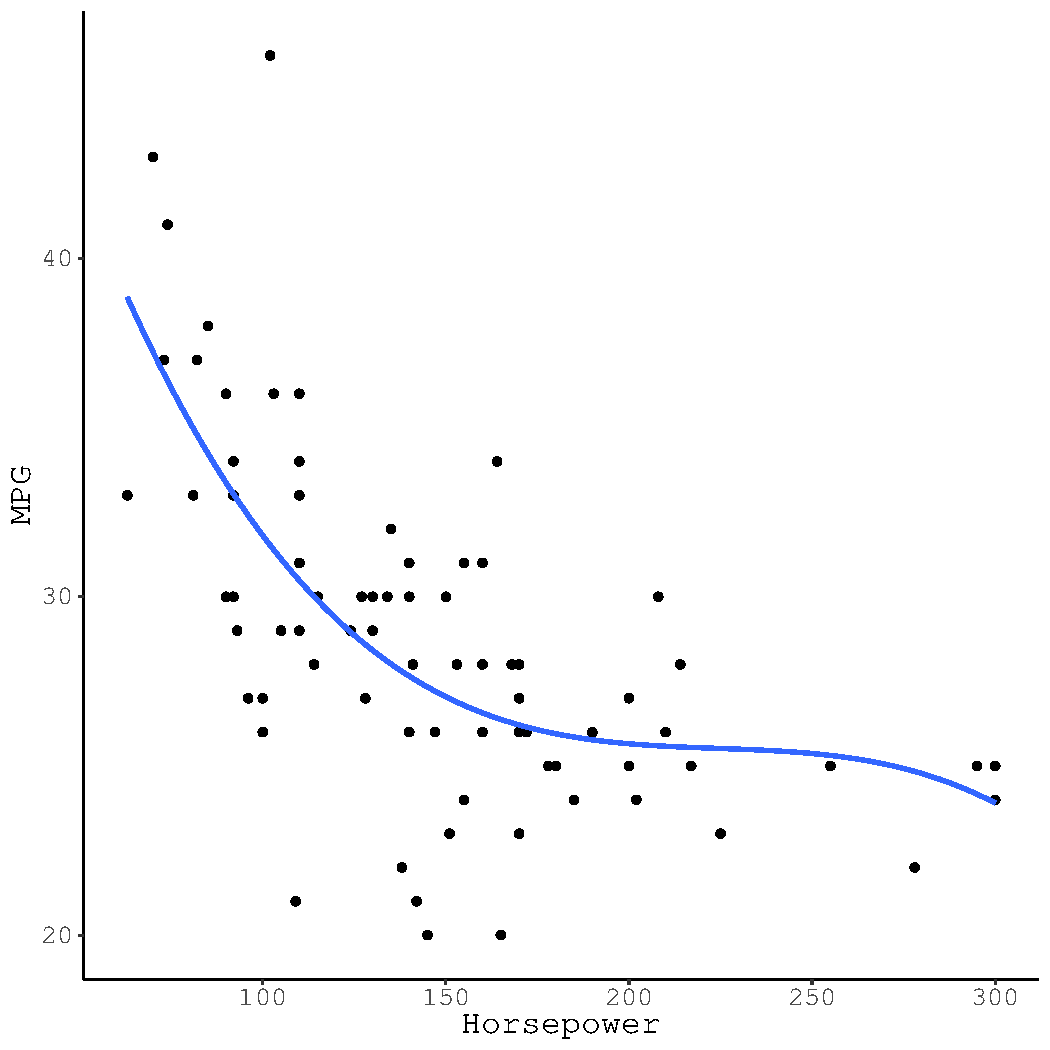
\includegraphics[width=\maxwidth]{figure/unnamed-chunk-47-1} 

}



\end{knitrout}

\end{column}

\begin{column}{0.5\textwidth}
  
\begin{knitrout}\footnotesize
\definecolor{shadecolor}{rgb}{0.878, 0.918, 0.933}\color{fgcolor}

{\centering 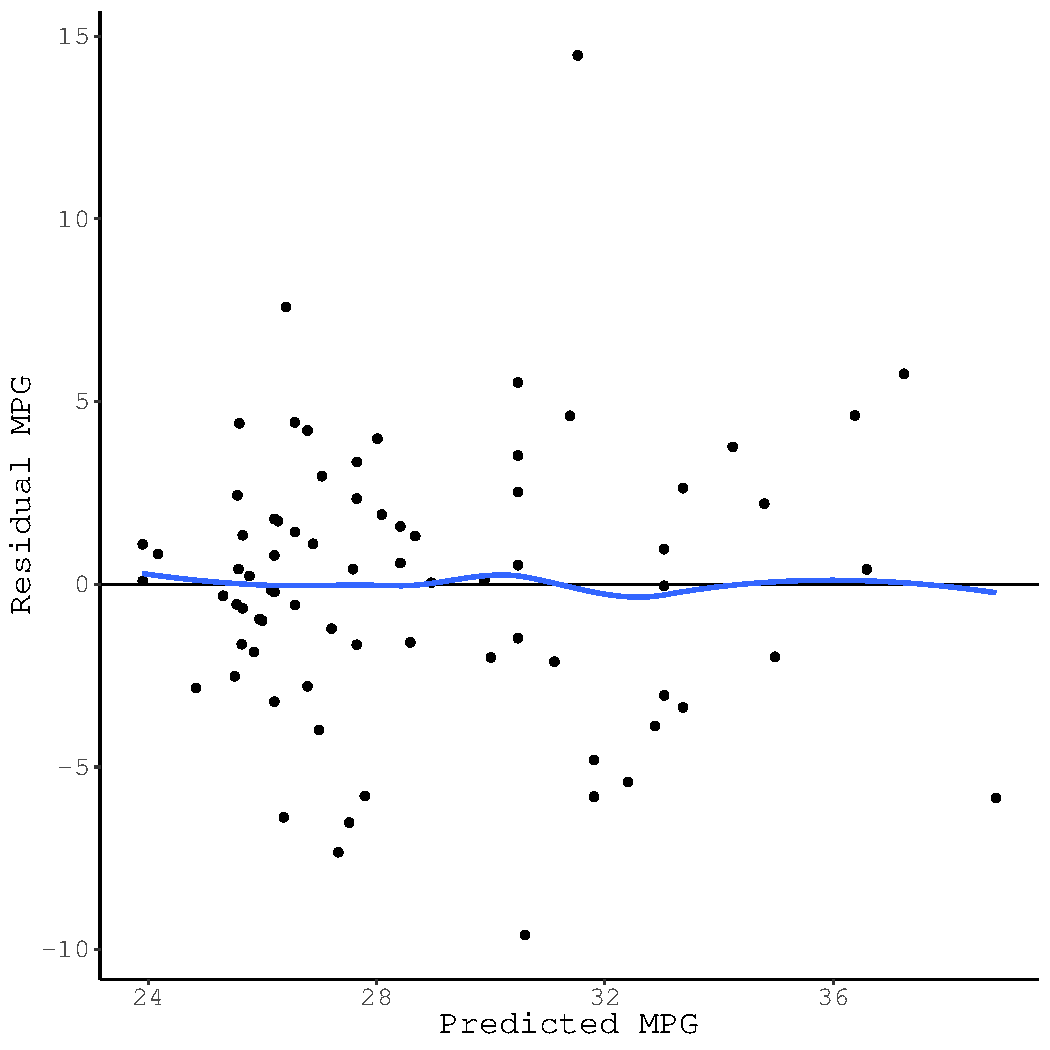
\includegraphics[width=\maxwidth]{figure/unnamed-chunk-48-1} 

}



\end{knitrout}

\end{column}
\end{columns}
  
\end{frame}

\watermarkon %-----------------------------------------------------------------%

\begin{frame}{Treating Influential Points}
  
  The most common way to address influential observations is simply to delete 
  them and refit the model.  
  \vc
  \begin{itemize}
  \item This approach is often effective---and always simple---but it is not
    fool-proof.
  \vc
  \item Although an observation is influential, we may not be able to justify 
    excluding it from the analysis.
  \end{itemize}
  \vb 
  Robust regression procedures can estimate the model directly in the
  presence of influential observations.  
  \vc
  \begin{itemize}
  \item Observations in the tails of the distribution are weighted less in the
    estimation process, so outliers and high-leverage points cannot exert
    substantial influence on the fit.
  \end{itemize}
  
\end{frame}

%------------------------------------------------------------------------------%

\begin{frame}[allowframebreaks]{Conclusion}
  
  \begin{itemize}
  \item The Gauss-Markov Theorem ensures that, when the assumptions are met, OLS 
    is the BLUE of a linear regression model.
    \begin{itemize}
    \item No other unbiased estimator will have lower variance than OLS.
    \end{itemize}
    \vb
  \item We stated the usual assumptions of OLS regression as:
    \begin{enumerate}
    \item The model is linear in the parameters.
    \item The predictor matrix is full rank.
    \item The predictors are strictly exogenous.
    \item The errors have constant, finite variance.
    \item The errors are uncorrelated.
    \item The errors are normally distributed.
    \end{enumerate}
    \vb
  \item Endogenous predictors will bias parameter estimates.
    \begin{itemize}
    \item Omitted variables
    \item Measurement error
    \end{itemize}
    
    \pagebreak
    
  \item Non-spherical errors will bias standard errors.
    \begin{itemize}
    \item Parameter estimates will remain unbiased.
    \end{itemize}
    \vb
  \item Non-normally distributed errors limit our inferential abilities.
    \vb
  \item We use regression diagnostics to check the model assumptions and find 
    influential observations.
    \vb
  \item Influential observations come in two flavors:
    \begin{enumerate}
    \item Outliers
    \item High-leverage points
    \end{enumerate}
    \vb
  \item Measures of influence combine outlier checks and leverage checks to find 
    highly influential observations.
    \begin{itemize}
    \item Measures of influence can be global or parameter-specific.
    \end{itemize}
  \end{itemize}
  
\end{frame}

%------------------------------------------------------------------------------%

\begin{frame}[allowframebreaks]{References}
  
  \bibliographystyle{apacite}
  \bibliography{../../../literature/bibtexFiles/statMethRefs.bib}
  
\end{frame}


%------------------------------------------------------------------------------%

\end{document}

